\documentclass[12pt,oneside]{book}

% --------------------
% Preamble / packages
% --------------------
\usepackage[a4paper,margin=1in]{geometry}
\usepackage{setspace}
\onehalfspacing
\usepackage{float}
\usepackage[T1]{fontenc}
\usepackage[utf8]{inputenc}
\usepackage{lmodern}
% Bold small-caps fallback for lmr (substitute bold upright); deferred so the
% lmr font family is fully registered before we declare the substitution shape.
\AtBeginDocument{\DeclareFontShape{T1}{lmr}{bx}{sc}{<->ssub*lmr/bx/n}{}}
\usepackage{graphicx}
\usepackage{amsmath,amssymb}
\usepackage{booktabs}
\usepackage{multirow}
\usepackage{tabularx}
\usepackage{caption}
\usepackage{subcaption}
\usepackage{enumitem}
\usepackage{xcolor}
\usepackage{pifont}

\usepackage[edges]{forest}
\usepackage{pdflscape}
\usepackage{rotating}   % sidewaysfigure: rotated full-page float without a clearpage gap
\usepackage{adjustbox}

\usepackage{algorithm}
\usepackage{algpseudocode}

\usepackage[numbers]{natbib}
\bibliographystyle{plainnat}

\usepackage[hidelinks]{hyperref}
\usepackage[nameinlink]{cleveref}
\usepackage{pdflscape}
\usepackage{tikz}
\usetikzlibrary{positioning, arrows.meta, fit, backgrounds, shapes.geometric, calc, decorations.pathreplacing, shadows.blur}

% ============================================================
% Shared visual system for all figures/charts
% ============================================================
\usepackage{pgfplots}
\pgfplotsset{compat=1.18}
\usepgfplotslibrary{groupplots}

% --- Unified colour palette (print-friendly, consistent across every figure) ---
\definecolor{svInk}{HTML}{1A2330}   % near-black ink (text, arrows)
\definecolor{svBlue}{HTML}{21487A}  % primary
\definecolor{svBlueT}{HTML}{DBE5F1} % primary tint (fill)
\definecolor{svOrange}{HTML}{E07B2C}% accent — "our method" highlight
\definecolor{svOrangeT}{HTML}{FAE6D2}
\definecolor{svTeal}{HTML}{2C7A7B}  % secondary data series
\definecolor{svTealT}{HTML}{D6E8E8}
\definecolor{svGreen}{HTML}{4F8A4C} % "good"/context
\definecolor{svGreenT}{HTML}{E1EFDD}
\definecolor{svGray}{HTML}{8A9099}  % neutral / baselines
\definecolor{svGrayT}{HTML}{ECEEF1}
\definecolor{svRed}{HTML}{C0504D}   % "bad"/greedy
\definecolor{svRedT}{HTML}{F6DEDD}

% --- Shared pgfplots base style ---
\pgfplotsset{
  sv base/.style={
    font=\small,
    axis line style={svGray, line width=0.6pt},
    tick style={svGray, line width=0.6pt},
    tick align=outside,
    label style={font=\small, text=svInk},
    tick label style={font=\footnotesize, text=svInk},
    title style={font=\bfseries, text=svInk},
    grid style={svGrayT, line width=0.5pt},
    legend style={font=\footnotesize, draw=svGrayT, fill=white,
                  /tikz/every even column/.append style={column sep=8pt}},
    nodes near coords style={font=\scriptsize, text=svInk},
  },
}

% --- Shared taxonomy node styles (used by the overview + the three branch figures) ---
\tikzset{
  taxroot/.style={fill=svBlue,   draw=svBlue,  text=white, font=\bfseries},
  taxuser/.style={fill=svOrangeT, draw=svOrange, line width=0.9pt, font=\bfseries},
  taxcomp/.style={fill=svBlueT,   draw=svBlue,   line width=0.9pt, font=\bfseries},
  taxsys/.style={ fill=svGreenT,  draw=svGreen,  line width=0.9pt, font=\bfseries},
  taxnew/.style={label={[fill=svGreenT, draw=svGreen, text=svGreen, font=\tiny\bfseries,
                 rounded corners=1.5pt, inner sep=1.5pt, xshift=-0.4cm, yshift=-0.1cm]above right:\textsc{new}}},
}

% --------------------
% Thesis metadata (edit these)
% --------------------
\newcommand{\ThesisTitle}{Smart Visit Module for Personalized Tourist Itinerary Recommendation Based on User Preferences and Contextual Data}
\newcommand{\ThesisAuthor}{Ayman Naaimi}
\newcommand{\ThesisDegree}{Master's Thesis}
\newcommand{\ThesisProgram}{D2SM}
\newcommand{\ThesisUniversity}{Ensam Meknes}
\newcommand{\ThesisYear}{2026}
\newcommand{\ThesisSupervisor}{IMADEDDINE MOUNTASSER}

% Convenience
\newcommand{\RQ}[1]{\textbf{RQ#1.}}

\begin{document}

% --------------------
% Front matter
% --------------------
\frontmatter
\begin{titlepage}
  \centering
  \vspace*{1.5cm}
  {\Large \ThesisUniversity \par}
  \vspace{1.0cm}
  {\Large \ThesisProgram \par}
  \vspace{1.8cm}
  {\Huge \bfseries \ThesisTitle \par}
  \vspace{2.0cm}
  {\Large \ThesisDegree \par}
  \vspace{1.0cm}
  {\Large \ThesisAuthor \par}
  \vfill
  {\large Supervisor: \ThesisSupervisor \par}
  \vspace{0.5cm}
  {\large \ThesisYear \par}
\end{titlepage}

\chapter*{Abstract}
\addcontentsline{toc}{chapter}{Abstract}
This thesis develops a personalized, context-aware engine for tourist recommendation and
decodes it into ordered itineraries, treating two \emph{formally distinct} sub-tasks and
evaluating each on its own field-standard benchmark. \textbf{Phase~1} is next-POI prediction:
a compact engine combining a graph convolutional network (GCN) over a hybrid point-of-interest
(POI) graph, per-step spatial and temporal gap features ($\Delta d$, $\Delta t$), a learnable
user embedding, and a gated-recurrent-unit (GRU) scorer, trained on the Foursquare NYC
check-in dataset and evaluated with full-vocabulary ranking metrics (HR@$k$, NDCG@$k$, MRR).
\textbf{Phase~2} is itinerary recommendation: the \emph{frozen} engine is decoded into ordered,
loop-free routes by a constraint-respecting rollout (\emph{Frozen Rollout}) and compared
against a pointer network trained end-to-end (\emph{Trained Pointer}), using the order-aware
pairs-F1 metric. Because the Foursquare itinerary scores are not on the same scale as the
published trip-recommendation literature, the task is re-validated on the Flickr
photo-trajectory datasets under the exact Chen-2016 protocol. The engine attains an honest
LSTM/STGCN-tier accuracy (HR@1 = 0.187); decoding the frozen engine \emph{outperforms} the
purpose-trained pointer (0.289 vs.\ 0.259 pairs-F1), a supervision-density effect rather than
an integration win; on the Flickr benchmark a Random baseline reproduces Chen 2016 (confirming
protocol faithfulness), our methods land on the published $0.26$--$0.85$ scale, and
personalization from the user embedding is beneficial but conditional. The contribution is an
honest, reproducible next-POI engine, a simple yet strong decoding method for itineraries, and
a literature-grounded benchmark that places both on a defensible footing.

\chapter*{Keywords}
\addcontentsline{toc}{chapter}{Keywords}
Tourism recommender systems; next-POI recommendation; itinerary recommendation; sequential recommendation; graph neural networks; context-aware recommendation; trajectory learning; pairs-F1.

\chapter*{Acknowledgements}
\addcontentsline{toc}{chapter}{Acknowledgements}
I would like to express my sincere gratitude to my supervisor, \ThesisSupervisor, for the
guidance, encouragement, and constructive feedback that shaped this work from its first
formulation to its final form. I am grateful to the faculty and staff of \ThesisUniversity\ and
the \ThesisProgram\ programme for the knowledge and the environment that made this research
possible. I also thank the authors of the open datasets and open-source tools used in this
thesis---in particular the Foursquare and Flickr trajectory benchmarks---without which the
experimental study could not have been carried out. Finally, I thank my family and friends for
their patience and unwavering support throughout this journey.

\tableofcontents
\listoffigures
\listoftables

\chapter*{List of Abbreviations}
\addcontentsline{toc}{chapter}{List of Abbreviations}
\begin{tabular}{@{}ll@{}}
CARS & Context-Aware Recommender Systems \\
POI  & Point of Interest \\
LBSN & Location-Based Social Network \\
GNN  & Graph Neural Network \\
GCN  & Graph Convolutional Network \\
GRU  & Gated Recurrent Unit \\
RNN  & Recurrent Neural Network \\
LSTM & Long Short-Term Memory \\
MLP  & Multilayer Perceptron \\
HR@$k$  & Hit Rate at $k$ \\
NDCG & Normalized Discounted Cumulative Gain \\
MRR  & Mean Reciprocal Rank \\
CF   & Collaborative Filtering \\
MF   & Matrix Factorization \\
RL   & Reinforcement Learning \\
LLM  & Large Language Model \\
TTDP & Tourist Trip Design Problem \\
OP   & Orienteering Problem \\
\end{tabular}

% --------------------
% Main matter
% --------------------
\mainmatter

\chapter{General Introduction}
\label{ch:introduction}

% ============================================================
\section{Background and Motivation}
\label{sec:intro-background}
% ============================================================

Tourism is one of the world's largest economic sectors. According to the World Travel and Tourism Council, the global travel and tourism industry contributed approximately USD~9.9 trillion to the world economy in 2023, accounting for roughly 9.1\% of global GDP and supporting over 320~million jobs worldwide~\cite{wttc2024}. Beyond its economic significance, tourism plays a central role in cultural exchange, urban development, and regional growth, with both developed and developing nations relying on tourism flows to sustain local economies and communities~\cite{unwto2024}.

The rapid expansion of digital technologies has fundamentally transformed how travelers plan and experience their journeys. Location-based social networks (LBSNs) such as Foursquare, TripAdvisor, and Google Maps now provide unprecedented volumes of user-generated data---check-ins, reviews, photographs, and ratings---that capture patterns of mobility and preference at a global scale~\cite{werneck2021poi}. At the same time, the proliferation of mobile devices equipped with GPS, real-time connectivity, and contextual sensors (e.g., weather, time, and location awareness) has created new opportunities for delivering personalized travel assistance at the point of need.

However, this abundance of information also creates a significant challenge for tourists. A major city may contain thousands of candidate points of interest (POIs) spanning museums, landmarks, restaurants, parks, cultural sites, and entertainment venues. Selecting which places to visit, in what order, and under what conditions is a combinatorial planning task that most travelers find cognitively overwhelming~\cite{gavalas2014ttdp}. Traditional travel planning tools---guidebooks, curated lists, and generic online platforms---typically recommend popular locations without accounting for individual preferences, time constraints, or real-time contextual factors such as weather or crowd conditions~\cite{lim2018survey}. This gap between the richness of available data and the difficulty of translating it into actionable, personalized travel plans motivates the development of intelligent tourism recommender systems.

% --- From POI recommendation to itinerary recommendation ---

Recommender systems have been extensively studied across domains such as e-commerce, media, and social platforms~\cite{koren2009mf}. In the tourism context, a substantial body of research has focused on \emph{point-of-interest (POI) recommendation}: given a user and their context, the system produces a ranked list of individual venues that the user is likely to enjoy~\cite{werneck2021poi, islam2022deep}. While POI recommendation is a valuable building block, it addresses only the question of \emph{what} to visit, not \emph{how} to visit it. In practice, tourists do not consume recommendations as isolated items. A city visit is inherently sequential and resource-constrained: a traveler typically has a limited time budget (e.g., a half-day or full day), must account for travel effort between locations, and often seeks a balanced and diverse set of experiences.

This observation motivates \emph{itinerary recommendation}, where the output is an ordered sequence of POIs forming an actionable, executable route---not merely a set of standalone suggestions~\cite{gavalas2014ttdp, halder2022thesis}. Itinerary recommendation is closely related to the Tourist Trip Design Problem (TTDP) and the Orienteering Problem (OP) in operations research, which explicitly model the selection and ordering of visits under time and travel constraints~\cite{vansteenwegen2011op}. However, classical optimization formulations typically rely on fixed, non-personalized utility scores (e.g., global popularity) and do not account for the dynamic, context-dependent nature of tourist preferences.

% --- Context-awareness ---

Tourist preferences are strongly context-dependent. The suitability of an activity changes with the time of day (morning visits to markets versus evening dining), weather conditions (outdoor landmarks versus indoor museums during rain), seasonal events, and even the traveler's energy level as a trip progresses. Context-aware recommender systems (CARS) formalize this dependence by extending the classical user--item relevance function to incorporate situational factors, estimating relevance as a function of user, item, and context~\cite{adomavicius2005cars, adomavicius2022cars, villegas2018cars}. Surveys on CARS demonstrate that explicitly modeling context can significantly improve recommendation relevance when contextual effects are present~\cite{raza2019cars}. In tourism, context is not only a preference signal but also a feasibility factor: weather and time influence both what a tourist \emph{wants} to do and what is \emph{practically possible} within a given itinerary.

% --- Evolution of approaches ---

The computational approaches for tourism recommendation have evolved considerably over the past decade. Early methods relied on collaborative filtering, matrix factorization, and content-based techniques adapted from general recommendation research~\cite{koren2009mf, burke2002hybrid}. The operations research community contributed optimization-based formulations that ensure feasibility but often lack personalization~\cite{vansteenwegen2011op, gavalas2014ttdp}. More recently, deep learning techniques have demonstrated superior performance in capturing complex user--POI interactions. Recurrent neural networks (RNNs) and their variants (GRU, LSTM) model sequential check-in behavior~\cite{liu2016strnn}, attention mechanisms and Transformer architectures capture long-range dependencies in visit sequences~\cite{sun2019bert4rec, kang2018sasrec}, graph neural networks (GNNs) encode spatial and social relationships between POIs~\cite{gnnpoi2024survey}, and reinforcement learning enables dynamic itinerary optimization~\cite{halder2022thesis, halder2025drlir}. Most recently, large language models (LLMs) have emerged as a new paradigm for travel planning, offering natural-language preference understanding and zero-shot recommendation capabilities, though they still struggle with constraint satisfaction and logistical feasibility~\cite{xie2024travelplanning, fan2024travelagent}.

Despite this progress, building a practical itinerary recommender that is simultaneously \emph{personalized}, \emph{context-aware}, and \emph{feasible} remains an open challenge. Most existing approaches address only a subset of these requirements: optimization methods ensure feasibility but lack personalization; sequential deep learning models capture preferences but produce infeasible routes when decoded greedily; and LLM-based planners understand user intent but cannot reliably satisfy hard constraints. Figure~\ref{fig:intro-overview} illustrates how this thesis positions the proposed system relative to these existing paradigms. This thesis aims to address this gap.

\begin{figure}[t]
\centering
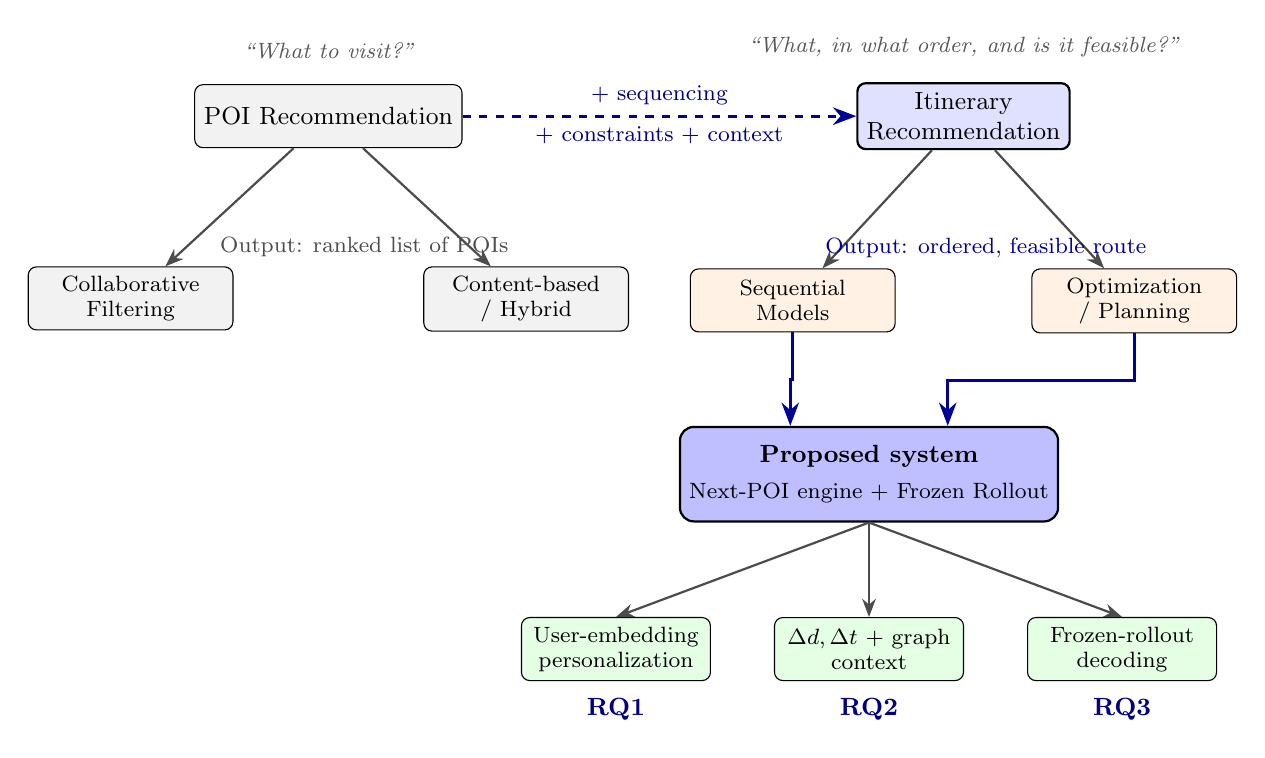
\begin{tikzpicture}[
    >=Stealth,
    node distance=1.2cm and 1.5cm,
    box/.style={draw, rounded corners=3pt, minimum width=2.6cm, minimum height=0.8cm, 
                align=center, font=\small},
    mainbox/.style={box, fill=blue!12, thick},
    graybox/.style={box, fill=gray!10},
    greenbox/.style={box, fill=green!10},
    orangebox/.style={box, fill=orange!10},
    label/.style={font=\footnotesize\itshape, text=gray!70!black},
    arrow/.style={->, thick, gray!60!black},
    darrow/.style={->, thick, blue!60!black, dashed},
]

% --- Left: POI Recommendation ---
\node[graybox] (poi) {POI Recommendation};
\node[label, above=0.2cm of poi] (poilabel) {``What to visit?''};

% Sub-nodes for POI
\node[graybox, below left=1.5cm and -0.5cm of poi] (cf) {\footnotesize Collaborative\\[-2pt] \footnotesize Filtering};
\node[graybox, below right=1.5cm and -0.5cm of poi] (cb) {\footnotesize Content-based\\[-2pt] \footnotesize / Hybrid};

\draw[arrow] (poi) -- (cf);
\draw[arrow] (poi) -- (cb);

% Output Label (Positioned between POI and its children)
\node[font=\footnotesize, text=gray!60!black, anchor=center] at ($(poi)!0.5!(cb)-(0.8,0.5)$) {Output: ranked list of POIs};

% --- Right: Itinerary Recommendation ---
\node[mainbox, right=5cm of poi] (itin) {Itinerary\\Recommendation};
\node[label, above=0.2cm of itin] (itinlabel) {``What, in what order, and is it feasible?''};

% Sub-nodes for Itinerary
\node[orangebox, below left=1.5cm and -0.5cm of itin] (seq) {\footnotesize Sequential\\[-2pt] \footnotesize Models};
\node[orangebox, below right=1.5cm and -0.5cm of itin] (opt) {\footnotesize Optimization\\[-2pt] \footnotesize / Planning};

\draw[arrow] (itin) -- (seq);
\draw[arrow] (itin) -- (opt);

% Output Label
\node[font=\footnotesize, text=blue!60!black, anchor=center] at ($(itin)!0.5!(opt)-(0.8,0.5)$) {Output: ordered, feasible route};

% --- Connection: POI to Itinerary ---
\draw[darrow, very thick] (poi.east) -- node[above, font=\footnotesize, text=blue!50!black] {+ sequencing} 
                                      node[below, font=\footnotesize, text=blue!50!black] {+ constraints + context} (itin.west);

% --- Proposed-system box (Centered below the itinerary branches) ---
\node[draw, thick, rounded corners=5pt, fill=blue!25, minimum width=4.5cm, minimum height=1.2cm,
      below=3.5cm of itin, xshift=-1.2cm, align=center, font=\small\bfseries] (sv) {Proposed system\\[2pt] \footnotesize\normalfont Next-POI engine + Frozen Rollout};

% Arrows into Smart Visit
\draw[->, very thick, blue!60!black] (seq.south) -- ++(0,-0.6) -| ([xshift=-1cm]sv.north);
\draw[->, very thick, blue!60!black] (opt.south) -- ++(0,-0.6) -| ([xshift=1cm]sv.north);

% --- Three pillars under the proposed system ---
\node[greenbox, below=1.2cm of sv, minimum width=2.4cm] (p2) {\footnotesize $\Delta d,\Delta t$ + graph\\[-2pt] \footnotesize context};
\node[greenbox, left=0.8cm of p2, minimum width=2.4cm] (p1) {\footnotesize User-embedding\\[-2pt] \footnotesize personalization};
\node[greenbox, right=0.8cm of p2, minimum width=2.4cm] (p3) {\footnotesize Frozen-rollout\\[-2pt] \footnotesize decoding};

\draw[arrow] (sv.south) -- (p1.north);
\draw[arrow] (sv.south) -- (p2.north);
\draw[arrow] (sv.south) -- (p3.north);

% --- RQ labels ---
\node[below=0.1cm of p1, font=\small\bfseries, text=blue!50!black] {RQ1};
\node[below=0.1cm of p2, font=\small\bfseries, text=blue!50!black] {RQ2};
\node[below=0.1cm of p3, font=\small\bfseries, text=blue!50!black] {RQ3};

\end{tikzpicture}
\caption{Positioning of the proposed system in the itinerary recommendation landscape.}
\label{fig:intro-overview}
\end{figure}


% ============================================================
\section{Research Aims}
\label{sec:intro-aims}
% ============================================================

The central objective of this thesis is to design and evaluate a personalized, context-aware \emph{next-POI engine} and a method for \emph{decoding} it into tourist itineraries. Unlike approaches that recommend isolated POIs, the system produces a \emph{complete ordered sequence} of visits, obtained by rolling the trained engine forward under loop-free and budget constraints.

For the next-POI task, the engine takes as input: (i)~a session prefix (the POIs visited so far), (ii)~per-step spatial and temporal gap features ($\Delta d$, the distance moved between consecutive visits, and $\Delta t$, the time elapsed), and (iii)~a user identifier encoded as a learnable embedding, all grounded in a city POI catalogue with a graph over its venues. For the itinerary task, a query additionally fixes a start POI, an optional end POI, and a length budget, and the output is an ordered, loop-free route over the catalogue.

This aim is approached through a deliberately \emph{decoupled} design: rather than training one monolithic itinerary generator, the thesis trains a strong next-POI model and obtains itineraries by decoding it. The engine combines (i)~a graph convolutional encoder over a hybrid POI graph, (ii)~spatial/temporal gap context, (iii)~a learnable user embedding for personalization, and (iv)~a GRU sequential backbone with a full-vocabulary scoring head; itineraries are then produced by \emph{Frozen Rollout} and compared against an end-to-end \emph{Trained Pointer}. Explicit weather and time-of-day context, persona-based cold-start, and penalty-augmented constrained decoding are promising extensions discussed as future work rather than claimed in the experiments.


% ============================================================
\section{Research Questions, Objectives, and Contributions}
\label{sec:intro-rqs}
% ============================================================

To achieve the aims described above, this thesis addresses three research questions, each targeting a specific challenge in personalized itinerary recommendation. For each question, we state the corresponding objective and the contribution made by this work.

% --- RQ1 ---
\subsection{RQ1: Personalization under Sparse Tourist Histories}
\label{sec:intro-rq1}

\textbf{Research Question 1.} \textit{Can a learnable per-user representation personalize tourist recommendation, and under what conditions does it help given the sparse, cold-start nature of tourist histories?}

\medskip

Tourism recommendation frequently operates under sparsity: a visitor may have few interactions in the destination city, and collaborative methods that rely on co-visitation degrade under such conditions~\cite{koren2009mf}. When personalization fails, systems fall back on globally popular POIs, producing homogeneous outputs that ignore individual interests.

\textbf{Objective.} Incorporate a user representation into the sequential engine and \emph{measure} its effect, isolating the contribution of identity-based personalization rather than assuming it always helps.

\textbf{Contribution.} We integrate a learnable user embedding into the engine and quantify its effect with a controlled on/off ablation. The finding is honest and \emph{conditional}: personalization helps where a user's signal is present and consistent (a clear gain on Glasgow) but is roughly neutral elsewhere under leave-one-trajectory-out evaluation---a cold-start effect on datasets with few trajectories per user. A richer persona/content-based representation that personalizes from explicit preferences and POI metadata, and a tourism-specific semantic curation of the catalogue, are identified as directions for future work.

% --- RQ2 ---
\subsection{RQ2: Spatial--Temporal Context for Sequential Prediction}
\label{sec:intro-rq2}

\textbf{Research Question 2.} \textit{How do spatial and temporal gap features between consecutive visits, together with a graph over POIs, improve sequential next-POI prediction?}

\medskip

Successive tourist visits are governed by how far and how long a person moves between venues; modelling these spatio-temporal regularities improves next-POI prediction over context-agnostic sequence models~\cite{liu2016strnn}. POIs are also related both spatially and behaviourally, structure that a graph can capture beyond each venue's identity~\cite{adomavicius2005cars, adomavicius2022cars}.

\textbf{Objective.} Condition the sequential model on per-step spatial ($\Delta d$) and temporal ($\Delta t$) gaps, and encode POIs with a graph neural network over a hybrid co-visitation/geographic graph, using shared representations that avoid the data fragmentation of context pre-filtering.

\textbf{Contribution.} We design a context-aware engine in which a two-layer GCN over a hybrid POI graph produces venue features, small MLPs lift the $(\Delta d,\Delta t)$ gaps into a context vector, and a GRU consumes their concatenation. This yields an honest LSTM/STGCN-tier accuracy on Foursquare NYC. Explicit environmental context (weather) and absolute time-of-day are deliberately not modelled and are left as future work---a scoping decision rather than a claimed capability~\cite{villegas2018cars, raza2019cars}.

% --- RQ3 ---
\subsection{RQ3: From Next-POI Prediction to Itineraries}
\label{sec:intro-rq3}

\textbf{Research Question 3.} \textit{Can a sequential next-POI model be decoded into complete, loop-free itineraries, and does training a dedicated itinerary model outperform decoding the frozen next-POI model?}

\medskip

Sequential models are trained for next-step prediction and evaluated with ranking metrics, but deploying them with greedy decoding need not yield good itineraries. A locally optimal next-POI choice can produce globally poor routes: excessive back-and-forth travel (zigzag behaviour) and violations of the budget~\cite{wu2025trajectory}. This mismatch between next-step accuracy and itinerary-level quality---which we term the \emph{greedy trap}---is a fundamental challenge for learning-based itinerary generation. Figure~\ref{fig:greedy-trap} illustrates the problem.

% Save this as figures/fig-greedy-trap.tex
% Include in the introduction with:
%   % Save this as figures/fig-greedy-trap.tex
% Include in the introduction with:
%   \input{figures/fig-greedy-trap}
%
% Requires: \usepackage{tikz}
%           \usetikzlibrary{positioning, arrows.meta, decorations.pathreplacing, calc}

\begin{figure}[!ht]
\centering
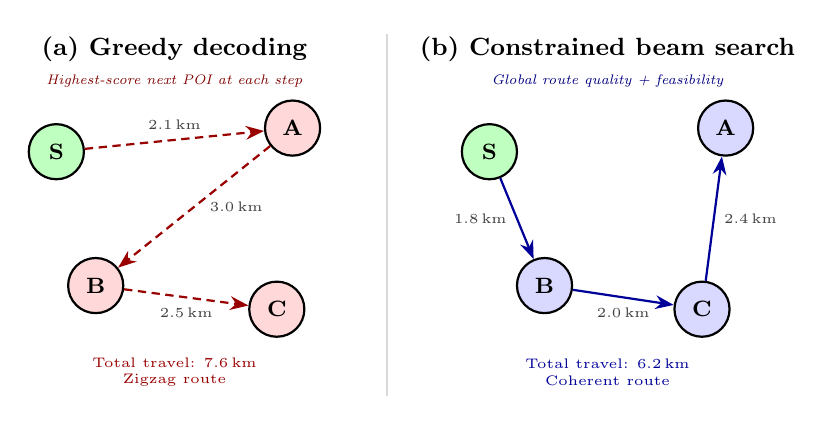
\begin{tikzpicture}[
    >=Stealth,
    poi/.style={circle, draw, thick, minimum size=0.7cm, font=\footnotesize\bfseries},
    start/.style={poi, fill=green!25},
    visit/.style={poi, fill=blue!15},
    visitbad/.style={poi, fill=red!15},
    label/.style={font=\tiny, text=gray!50!black},
    route/.style={->, thick},
    badroute/.style={->, thick, red!60!black, densely dashed},
    goodroute/.style={->, thick, blue!60!black},
]

% ---- Left: Greedy decoding (zigzag) ----
\node[font=\small\bfseries] at (1.5, 3.8) {(a) Greedy decoding};
\node[font=\tiny\itshape, text=red!50!black] at (1.5, 3.4) {Highest-score next POI at each step};

\node[start]   (gS) at (0, 2.5) {S};
\node[visitbad] (gA) at (3, 2.8) {A};
\node[visitbad] (gB) at (0.5, 0.8) {B};
\node[visitbad] (gC) at (2.8, 0.5) {C};

% Greedy path (zigzag)
\draw[badroute] (gS) -- (gA) node[midway, above, label] {2.1\,km};
\draw[badroute] (gA) -- (gB) node[midway, right, label, xshift=2pt] {3.0\,km};
\draw[badroute] (gB) -- (gC) node[midway, below, label] {2.5\,km};

% Total
\node[font=\tiny, text=red!60!black, align=center] at (1.5, -0.3) {Total travel: 7.6\,km\\Zigzag route};

% ---- Right: Constrained decoding (coherent) ----
\node[font=\small\bfseries] at (7, 3.8) {(b) Constrained beam search};
\node[font=\tiny\itshape, text=blue!50!black] at (7, 3.4) {Global route quality + feasibility};

\node[start]  (cS) at (5.5, 2.5) {S};
\node[visit]  (cB) at (6.2, 0.8) {B};
\node[visit]  (cC) at (8.2, 0.5) {C};
\node[visit]  (cA) at (8.5, 2.8) {A};

% Coherent path
\draw[goodroute] (cS) -- (cB) node[midway, left, label] {1.8\,km};
\draw[goodroute] (cB) -- (cC) node[midway, below, label] {2.0\,km};
\draw[goodroute] (cC) -- (cA) node[midway, right, label] {2.4\,km};

% Total
\node[font=\tiny, text=blue!60!black, align=center] at (7, -0.3) {Total travel: 6.2\,km\\Coherent route};

% --- Separator ---
\draw[gray!30, thick] (4.2, -0.6) -- (4.2, 4.0);

\end{tikzpicture}
\caption{Illustration of the ``greedy trap'' in itinerary generation. (a)~Greedy decoding selects the highest-scoring next POI at each step, resulting in a zigzag route with excessive travel. (b)~Constrained beam search considers global route quality, producing a geographically coherent itinerary visiting the same POIs with less travel cost.}
\label{fig:greedy-trap}
\end{figure}
%
% Requires: \usepackage{tikz}
%           \usetikzlibrary{positioning, arrows.meta, decorations.pathreplacing, calc}

\begin{figure}[!ht]
\centering
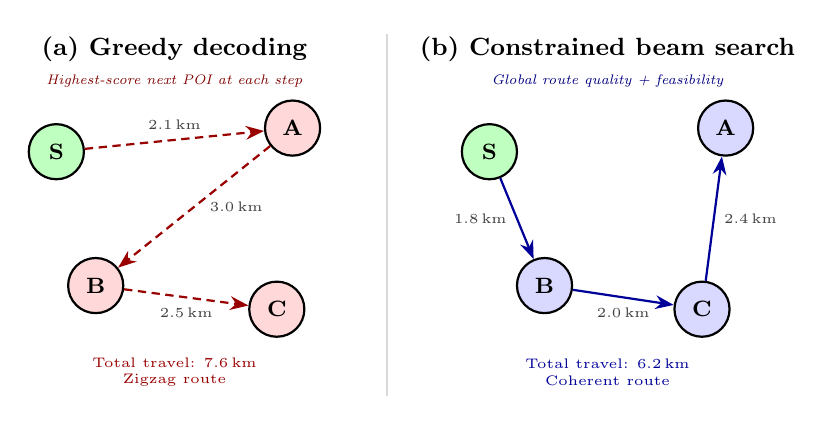
\begin{tikzpicture}[
    >=Stealth,
    poi/.style={circle, draw, thick, minimum size=0.7cm, font=\footnotesize\bfseries},
    start/.style={poi, fill=green!25},
    visit/.style={poi, fill=blue!15},
    visitbad/.style={poi, fill=red!15},
    label/.style={font=\tiny, text=gray!50!black},
    route/.style={->, thick},
    badroute/.style={->, thick, red!60!black, densely dashed},
    goodroute/.style={->, thick, blue!60!black},
]

% ---- Left: Greedy decoding (zigzag) ----
\node[font=\small\bfseries] at (1.5, 3.8) {(a) Greedy decoding};
\node[font=\tiny\itshape, text=red!50!black] at (1.5, 3.4) {Highest-score next POI at each step};

\node[start]   (gS) at (0, 2.5) {S};
\node[visitbad] (gA) at (3, 2.8) {A};
\node[visitbad] (gB) at (0.5, 0.8) {B};
\node[visitbad] (gC) at (2.8, 0.5) {C};

% Greedy path (zigzag)
\draw[badroute] (gS) -- (gA) node[midway, above, label] {2.1\,km};
\draw[badroute] (gA) -- (gB) node[midway, right, label, xshift=2pt] {3.0\,km};
\draw[badroute] (gB) -- (gC) node[midway, below, label] {2.5\,km};

% Total
\node[font=\tiny, text=red!60!black, align=center] at (1.5, -0.3) {Total travel: 7.6\,km\\Zigzag route};

% ---- Right: Constrained decoding (coherent) ----
\node[font=\small\bfseries] at (7, 3.8) {(b) Constrained beam search};
\node[font=\tiny\itshape, text=blue!50!black] at (7, 3.4) {Global route quality + feasibility};

\node[start]  (cS) at (5.5, 2.5) {S};
\node[visit]  (cB) at (6.2, 0.8) {B};
\node[visit]  (cC) at (8.2, 0.5) {C};
\node[visit]  (cA) at (8.5, 2.8) {A};

% Coherent path
\draw[goodroute] (cS) -- (cB) node[midway, left, label] {1.8\,km};
\draw[goodroute] (cB) -- (cC) node[midway, below, label] {2.0\,km};
\draw[goodroute] (cC) -- (cA) node[midway, right, label] {2.4\,km};

% Total
\node[font=\tiny, text=blue!60!black, align=center] at (7, -0.3) {Total travel: 6.2\,km\\Coherent route};

% --- Separator ---
\draw[gray!30, thick] (4.2, -0.6) -- (4.2, 4.0);

\end{tikzpicture}
\caption{Illustration of the ``greedy trap'' in itinerary generation. (a)~Greedy decoding selects the highest-scoring next POI at each step, resulting in a zigzag route with excessive travel. (b)~Constrained beam search considers global route quality, producing a geographically coherent itinerary visiting the same POIs with less travel cost.}
\label{fig:greedy-trap}
\end{figure}

\textbf{Objective.} Develop an inference-time procedure that turns the trained scorer into an itinerary planner, and test it against a purpose-trained alternative to determine whether end-to-end integration is worth its cost.

\textbf{Contribution.} We introduce \emph{Frozen Rollout}, which decodes the \emph{frozen} engine into ordered, loop-free routes using a no-revisit mask and a reserved end POI (greedy or beam search), and compare it against a \emph{Trained Pointer} trained end-to-end on whole trajectories. The central, somewhat counter-intuitive finding is that decoding the frozen engine \emph{outperforms} the purpose-trained pointer, because the next-POI model enjoys far denser supervision---nuancing the assumption that an integrated itinerary model is necessarily better. We further adopt a two-benchmark evaluation (full-vocabulary ranking metrics for next-POI; order-aware set-F1/pairs-F1 for itineraries, re-validated on the Flickr datasets), and identify penalty-augmented constrained decoding (travel-cost and diversity terms) as a natural extension left for future work.


% ============================================================
\section{Thesis Organization}
\label{sec:intro-organization}
% ============================================================

The remainder of this thesis is organized as follows.

\textbf{Chapter~\ref{ch:problem}} formalizes the itinerary recommendation problem addressed in this thesis. It specifies the inputs, outputs, and notation; defines hard feasibility constraints and soft quality objectives; discusses the key technical challenges (data bias, cold-start, and the greedy trap); and presents the research questions and evaluation perspective.

\textbf{Chapter~\ref{ch:sota}} provides a comprehensive state of the art in tourist itinerary and POI recommendation. The chapter is organized as a field taxonomy, covering non-personalized approaches (orienteering problems, general POI recommendation), personalized methods (collaborative filtering, content-based, hybrid), deep learning models (RNN, Transformer, GNN, reinforcement learning), context-aware recommendation, and emerging paradigms (LLM-based planning, self-supervised learning, fairness). The chapter concludes with a comparative synthesis and gap analysis mapped to the research questions.

\textbf{Chapter~\ref{ch:solution}} presents the proposed system in detail: the data preparation, the context-aware next-POI engine (a GCN over a hybrid POI graph, $(\Delta d,\Delta t)$ context, a user embedding, and a GRU scorer), the Frozen Rollout decoder and the Trained Pointer comparison, and the experimental evaluation---including the next-POI results, the NYC integration experiment, the literature-comparable Flickr benchmark, and the personalization ablation.

\textbf{Chapter~\ref{ch:conclusion}} concludes the thesis by summarizing findings, discussing limitations, and outlining directions for future work.
\chapter{Problem Definition}
\label{ch:problem}

\section{Context and Motivation}
\label{sec:prob-context}

Tourist recommendation has traditionally focused on suggesting \emph{individual} points of interest (POIs), such as attractions, museums, restaurants, or viewpoints. While these recommendations can be useful, they do not fully match the way tourists plan and experience a city visit. In practice, a visitor typically needs an \emph{itinerary}: a coherent sequence of POIs that can be executed within a limited time budget (e.g., a half-day or a full day), with reasonable travel effort between successive stops and a balance of experiences.

This thesis addresses itinerary recommendation as a problem at the intersection of (i) personalized recommendation and (ii) route planning. From a recommendation perspective, the system should adapt to user-specific interests and preferences, including cold-start scenarios where historical interaction data is limited or absent \citep{koren2009mf, burke2002hybrid}. From a context-aware perspective, suitability depends on situational factors such as \textbf{time-of-day} and \textbf{weather}, which can strongly influence what is appropriate or enjoyable (e.g., outdoor activities in good weather, indoor alternatives during rain). Context-aware recommender systems formalize this dependency by modeling relevance as a function of user, item, and context \citep{adomavicius2005tois, adomavicius2022cars, villegas2018cars}.

Unlike recommending a single POI, itinerary recommendation introduces additional structure and constraints. First, the output is inherently \emph{sequential}: the quality of a candidate POI depends not only on user preference but also on the already selected stops and their geographic placement. Second, itineraries must be \emph{feasible}: travel time and visit durations accumulate and must remain within a budget, and (when available) opening hours impose time-window constraints. These considerations connect the problem to tourism route planning formulations such as the Tourist Trip Design Problem (TTDP), where selecting and ordering locations is constrained by time and travel cost \citep{gavalas2014ttdp}.

Recent learning-based approaches for route-like or itinerary generation show the promise of sequential modeling for this task \citep{wu2025tlmr, chang2025itinerary, halder2025deeptourrec}. However, tourism settings pose additional challenges due to noisy and biased mobility data (e.g., resident-dominated check-ins or vehicle trajectories) and the gap between next-step prediction accuracy and long-horizon itinerary quality. These challenges motivate a careful problem formulation in which personalization, context-awareness, geographic coherence, and feasibility are treated as first-class objectives rather than secondary post-processing steps.

In the remainder of this chapter, we formalize the itinerary recommendation task addressed by the proposed system by specifying the inputs, outputs, constraints, and evaluation criteria, and by clarifying the key technical challenges that guide the research questions of this thesis.

\section{Problem Statement}
\label{sec:prob-statement}

The goal of the proposed system is to generate a \textbf{personalized and context-aware tourist itinerary} for a given city. In contrast to classic POI recommendation, which outputs a ranked list of venues, itinerary recommendation must output an \emph{ordered sequence} of POIs that forms a geographically coherent route and can be executed within real-world constraints such as limited time and travel cost \citep{gavalas2014ttdp}.

\paragraph{Informal statement.}
Given (i) a user description (persona and/or explicit preferences), (ii) the current context (time-of-day and weather), and (iii) a city POI catalog with geographic and semantic metadata, the system should recommend an itinerary that:
\begin{itemize}[leftmargin=*]
    \item matches the user's interests (personalization),
    \item is appropriate for the context (context-awareness),
    \item is geographically coherent (avoids unnecessary back-and-forth travel),
    \item respects feasibility constraints (time budget and travel cost),
    \item and provides a diverse set of experiences (avoids redundancy).
\end{itemize}

\paragraph{Motivating use case.}
A typical usage scenario is a visitor planning a \emph{half-day} or \emph{full-day} city tour. The visitor may provide high-level preferences (e.g., ``history'', ``architecture'', ``local food'', ``outdoor viewpoints'') and may have little to no historical interaction data in the target city (cold-start). The system then generates a multi-stop itinerary (e.g., 5--10 venues) that can realistically be followed given the available time and current conditions.

\paragraph{Scope of the problem in this thesis.}
This thesis focuses on \textbf{offline itinerary generation} from Foursquare-style POI data and historical mobility/check-in sequences. The objective is not only to predict the next POI in a trajectory, but to generate a \emph{complete itinerary} that is executable and coherent. In later chapters, we show how this requires going beyond greedy next-step prediction, since step-wise optimization can lead to infeasible or zigzag routes even when next-POI ranking accuracy is high \citep{wu2025tlmr}.


\section{Definitions and Notation}
\label{sec:prob-defs}

This section introduces the objects used to define the itinerary recommendation task and establishes a lightweight notation that will be reused in Chapters~\ref{ch:sota} and \ref{ch:solution}.

\subsection{Points of interest and city catalog}
Let a \textbf{point of interest (POI)} be a visitable venue such as an attraction, museum, restaurant, park, or landmark. For a given city, we denote the set of available POIs by $\mathcal{V}=\{v_1,\dots,v_{|\mathcal{V}|}\}$. Each POI $v \in \mathcal{V}$ is associated with:
\begin{itemize}[leftmargin=*]
    \item \textbf{Geographic location:} latitude/longitude coordinates $\mathrm{loc}(v)$,
    \item \textbf{Semantic attributes:} category labels and/or textual descriptors (e.g., tags, name, short description),
    \item \textbf{Popularity signals:} optional aggregate statistics such as total check-ins or visits,
    \item \textbf{Operational attributes (optional):} opening hours, price range, or estimated visit duration.
\end{itemize}

Since raw LBSN catalogs may contain many non-touristic venues (e.g., offices, local services), this thesis assumes that the city catalog can be transformed into a curated subset of \textbf{tourist-relevant POIs} via semantic filtering. We denote the curated set by $\mathcal{V}^{\star} \subseteq \mathcal{V}$. This curation step is motivated by dataset bias and noise typical of check-in data, where activity may reflect resident routines more than tourist intent.

\subsection{Users, personas, and preference representation}
Let $\mathcal{U}$ denote the set of users. A user can be represented in two complementary ways:
\begin{itemize}[leftmargin=*]
    \item \textbf{Interaction history} (when available): a sequence of previously visited POIs,
    \item \textbf{Explicit persona/preferences:} a high-level description of interests (e.g., ``culture'', ``food'', ``nature'').
\end{itemize}

To support cold-start settings, the thesis assumes that user interests can be encoded as a \textbf{preference vector} $\mathbf{p}_u \in \mathbb{R}^{d}$ derived from persona inputs and/or observed interactions. Hybrid recommendation is a common strategy for combining preference signals from content with collaborative patterns when available \citep{burke2002hybrid}. In the proposed framework (Chapter~\ref{ch:solution}), $\mathbf{p}_u$ is used as an explicit conditioning signal for itinerary generation.

\subsection{Context variables}
We define context as a set of situational variables observed at recommendation time. In the realized system, the contextual signal is the pair of \textbf{spatial and temporal gaps} between consecutive visits:
\begin{itemize}[leftmargin=*]
    \item \textbf{Spatial gap} $\Delta d_t$: the haversine distance moved from the previous POI,
    \item \textbf{Temporal gap} $\Delta t_t$: the time elapsed since the previous visit.
\end{itemize}
We denote the per-step context by $c_t \in \mathcal{C}$. Other situational factors---notably time-of-day and weather---fit the same context-aware formulation, in which relevance is modelled as a function of $(u,v,c)$ rather than $(u,v)$ only \citep{adomavicius2005tois, adomavicius2022cars, villegas2018cars}; they are identified as future extensions (Chapter~\ref{ch:conclusion}) rather than modelled in this thesis.

\subsection{Itineraries and travel cost}
An itinerary of length $L$ is an ordered sequence of POIs:
\[
\mathbf{s} = (s_1, s_2, \dots, s_L), \qquad s_{\ell} \in \mathcal{V}^{\star}.
\]
Optionally, an itinerary can be augmented with a schedule of visit start times $\mathbf{t}=(t_1,\dots,t_L)$, but the minimal output required by this thesis is the ordered POI sequence.

We model movement between POIs using a nonnegative \textbf{travel cost} function:
\[
\tau: \mathcal{V}^{\star} \times \mathcal{V}^{\star} \rightarrow \mathbb{R}_{\ge 0},
\]
which represents travel time or distance between two POIs. In practice, $\tau$ may be approximated using geographic distance or routing estimates. Additionally, each POI $v$ may have an estimated \textbf{visit duration} $\delta(v) \ge 0$, representing expected time spent at the venue.

These quantities are standard in itinerary planning and TTDP-style formulations, where the sequence must satisfy time and travel constraints \citep{gavalas2014ttdp}.

\section{Inputs, Outputs, and System Requirements}
\label{sec:prob-io}

This section specifies the information available to the system (inputs), the expected output, and the core requirements that define what a ``good'' itinerary means in the setting of this thesis.

\subsection{Inputs}
At recommendation time, the system receives the following inputs.

\paragraph{User representation.}
A user $u \in \mathcal{U}$ is represented by a preference signal. In cold-start settings, this signal is primarily derived from an explicit persona/preferences description and encoded as a vector $\mathbf{p}_u \in \mathbb{R}^d$ (see \Cref{sec:prob-defs}). When historical interactions are available, they can be used to refine this representation via hybrid modeling \citep{burke2002hybrid}.

\paragraph{Context.}
The system observes per-step situational context---in the realized engine, the spatial and temporal gaps $(\Delta d,\Delta t)$ between consecutive visits. We denote the context by $c \in \mathcal{C}$ (or $c_t$ at step $t$), following the context-aware recommendation formulation \citep{adomavicius2005tois, adomavicius2022cars}; time-of-day and weather fit the same formulation and are left as future extensions.

\paragraph{City POI catalog.}
The system has access to a city-specific POI set $\mathcal{V}$ with semantic and geographic metadata. Because raw catalogs can include many non-touristic venues and bias the learning signal toward resident routines, this thesis assumes the availability of a curated tourist-relevant subset $\mathcal{V}^{\star}\subseteq \mathcal{V}$ obtained through semantic pruning.

\paragraph{Operational parameters.}
The itinerary generation request includes operational constraints such as:
\begin{itemize}[leftmargin=*]
    \item \textbf{Time budget} $B$ (e.g., half-day or full-day),
    \item \textbf{Optional start location} (e.g., hotel area) and/or end location,
    \item \textbf{Optional constraints} such as maximum number of POIs $L_{\max}$ or category preferences.
\end{itemize}

\subsection{Outputs}
The primary output of the system is an itinerary:
\[
\mathbf{s} = (s_1, s_2, \dots, s_L), \qquad s_{\ell} \in \mathcal{V}^{\star},
\]
where $L$ may be fixed (e.g., requested length) or determined by the budget and constraints.

Optionally, the system may output auxiliary information to support interpretability and downstream use:
\begin{itemize}[leftmargin=*]
    \item \textbf{Estimated schedule:} visit start times $\mathbf{t}$ and/or per-stop durations,
    \item \textbf{Cost summary:} estimated travel time/distance and total itinerary duration,
    \item \textbf{Explanations:} a short justification for recommended POIs based on persona and context.
\end{itemize}
In this thesis, the core algorithmic output is the \emph{ordered POI sequence}; schedule generation is considered optional and can be approximated if opening hours are unavailable.

\subsection{System requirements}
We define the key requirements that a recommended itinerary should satisfy. These requirements guide both model design and evaluation.

\paragraph{R1: Personal relevance.}
The itinerary should match the user's interests, as encoded by $\mathbf{p}_u$. This requirement is particularly important under cold-start, where preferences must be inferred from persona-level signals rather than dense historical trajectories.

\paragraph{R2: Context suitability.}
The itinerary should be appropriate for the observed context (time-of-day and weather). Context influences both preference (what feels suitable) and feasibility (e.g., willingness to walk long distances in rain), which motivates explicit context-aware modeling \citep{adomavicius2005tois, adomavicius2022cars}.

\paragraph{R3: Geographic coherence.}
Successive POIs should form a coherent route with reasonable travel cost, avoiding unnecessary backtracking (zigzag behavior). Geographic coherence is a defining feature of itineraries and cannot be guaranteed by static POI ranking.

\paragraph{R4: Feasibility.}
The itinerary must respect hard operational constraints, primarily the time budget $B$ and travel cost accumulation. When available, additional constraints such as opening hours/time windows should also be respected.

\paragraph{R5: Diversity and non-redundancy.}
The itinerary should provide a balanced experience and avoid recommending multiple POIs that are too similar (e.g., repeated venues from the same narrow category) unless explicitly desired. Diversity improves user experience and reduces the tendency to recommend only the most popular venues.

Together, these requirements define itinerary quality in this problem: a high-quality itinerary is personalized, context-aware, feasible, coherent, and diverse.

\section{Constraints and Objective Formulation}
\label{sec:prob-constraints}

This section makes the feasibility requirements explicit and introduces a practical objective view of itinerary quality. The intent is not to impose a single rigid mathematical formulation, but to define the constraints and trade-offs that any solution must address.

\subsection{Hard feasibility constraints}
Let $\mathbf{s}=(s_1,\dots,s_L)$ be a candidate itinerary, where each $s_\ell \in \mathcal{V}^{\star}$. We consider the following hard constraints.

\paragraph{C1: Time budget constraint.}
Given a total available time budget $B$, an itinerary is feasible if the sum of visit durations and travel costs fits within $B$:
\[
T(\mathbf{s}) \;=\; \sum_{\ell=1}^{L}\delta(s_\ell) \;+\; \sum_{\ell=1}^{L-1}\tau(s_\ell, s_{\ell+1})
\;\;\le\;\; B.
\]
This is the central feasibility constraint in TTDP-style planning formulations \citep{gavalas2014ttdp}.

\paragraph{C2: Uniqueness constraint.}
A POI should not appear more than once in the same itinerary:
\[
s_i \neq s_j \quad \text{for all } i \neq j.
\]
This avoids trivial loops and improves interpretability.

\paragraph{C3: Bound on itinerary length (optional).}
In practical settings, a user may request a maximum number of stops $L_{\max}$:
\[
L \le L_{\max}.
\]
Even when $L_{\max}$ is not explicitly given, it can be derived from budget considerations (e.g., typical visit durations).

\paragraph{C4: Opening hours and time windows (optional).}
If opening hour data is available, each POI $v$ can be associated with an admissible visit interval $[a(v), b(v)]$.
A scheduled itinerary $(\mathbf{s},\mathbf{t})$ is feasible if each visit starts within its time window:
\[
t_\ell \in [a(s_\ell), b(s_\ell)] \quad \forall \ell,
\]
and travel and visit times are consistent:
\[
t_{\ell+1} \ge t_\ell + \delta(s_\ell) + \tau(s_\ell, s_{\ell+1}).
\]
Because opening hours are not always present in Foursquare-style datasets, this constraint is treated as optional in this thesis; however, the framework is designed such that it can be incorporated when such metadata is available.

\subsection{Soft objectives for itinerary quality}
Among feasible itineraries, the system must choose those that best satisfy user-centric quality objectives. We treat these objectives as \emph{soft} constraints: they guide optimization but can be traded off against each other.

\paragraph{O1: Preference alignment (personalization).}
An itinerary should maximize alignment with the user's preference representation $\mathbf{p}_u$. This alignment can be expressed through a per-POI relevance score $r(u, v, c)$ learned from data or derived from semantic similarity.

\paragraph{O2: Context alignment.}
The itinerary should be suitable for the observed context (time-of-day and weather). In practice, this can be captured by context-conditioned scoring (e.g., different relevance for the same POI under different $c$) \citep{adomavicius2005tois, adomavicius2022cars}.

\paragraph{O3: Geographic coherence and travel-effort minimization.}
Even when the budget constraint is satisfied, itineraries can differ significantly in travel effort. A coherent itinerary should avoid unnecessary long legs and excessive backtracking. This objective can be expressed through penalties based on travel costs, for example minimizing:
\[
\mathrm{Travel}(\mathbf{s}) = \sum_{\ell=1}^{L-1}\tau(s_\ell, s_{\ell+1}).
\]

\paragraph{O4: Diversity and experience balance.}
To avoid redundant experiences, itineraries should cover diverse categories or semantic themes. Diversity can be measured using category entropy or pairwise dissimilarity between POIs, and then treated as a reward.

\subsection{A practical multi-objective view}
Combining these components, a useful conceptual objective is to select an itinerary that maximizes a composite score of the form:
\[
\max_{\mathbf{s}} \;\;
\underbrace{\sum_{\ell=1}^{L} r(u, s_\ell, c_\ell)}_{\text{personal relevance + context}}
\;-\;
\lambda_{\mathrm{tr}} \underbrace{\sum_{\ell=1}^{L-1}\tau(s_\ell, s_{\ell+1})}_{\text{travel effort}}
\;+\;
\lambda_{\mathrm{div}} \underbrace{\mathrm{Div}(\mathbf{s})}_{\text{diversity}}
\]
subject to the hard feasibility constraints above.

This formulation makes two important points explicit. First, itinerary generation is inherently \textbf{multi-objective}: the best itinerary is not simply the one with the top-ranked individual POIs, but the one that jointly optimizes relevance, coherence, and diversity under constraints. Second, feasibility is not a post-processing detail: the set of valid itineraries is restricted by budget and operational constraints, which requires algorithms capable of reasoning over \emph{sequences} rather than independent POIs.

In the next section, we discuss why this problem remains challenging in practice, focusing on dataset bias, cold-start, and the limitations of greedy next-step recommendation.

\section{Key Challenges}
\label{sec:prob-challenges}

Although itinerary recommendation can be expressed using the constraints and objectives in \Cref{sec:prob-constraints}, solving the problem in realistic tourism settings is challenging. This section highlights the main difficulties that motivate the design choices of the proposed system and directly inform the research questions of this thesis.

\subsection{Bias and noise in mobility and check-in data}
A large portion of POI and trajectory modeling research relies on LBSN check-ins or mobility traces. These data sources provide valuable sequential signals but can be misaligned with the notion of ``tourist interest'' in at least three ways.

\paragraph{Resident dominance.}
Public check-in datasets often contain a high proportion of residents, and common preprocessing steps (e.g., keeping users with many check-ins) can further amplify routine mobility patterns. As a result, models may learn preferences and transitions that reflect daily habits (home/work neighborhoods, frequent convenience venues) rather than visitor exploration.

\paragraph{Mobility-mode bias (``taxi bias'').}
Trajectory datasets derived from vehicles (e.g., taxi traces) encode movement optimized for speed, road structure, and service demand. When such trajectories are used to learn route patterns, a model may prioritize transitions that are efficient for transportation rather than meaningful for sightseeing. This can lead to itineraries that appear ``coherent'' in travel-time terms but are not aligned with tourist utility.

\paragraph{Implicit feedback noise.}
Check-ins and location logs do not directly measure satisfaction: they can be influenced by platform usage habits, social signaling, or convenience rather than genuine preference. Consequently, raw interaction frequency can be a misleading proxy for tourist relevance.

These issues motivate the need for data curation (e.g., semantic pruning of tourist POIs) and for evaluation measures that reflect itinerary quality rather than only next-POI prediction accuracy.

\subsection{Cold-start personalization in tourism (\textbf{RQ1})}
Cold-start is a fundamental difficulty in tourist recommendation. Many visitors have little to no interaction history in the target city, and even when a user has general history elsewhere, their preferences may not be well represented in the local POI catalog. This produces several practical cold-start regimes:
\begin{itemize}[leftmargin=*]
    \item \textbf{New user:} no interaction history; personalization must rely on explicit persona/preferences.
    \item \textbf{New city/session:} user history exists but is sparse for the target city.
    \item \textbf{Sparse POI observations:} long-tail tourist venues may have limited check-ins.
\end{itemize}
Collaborative filtering methods are known to degrade in sparse regimes \citep{koren2009mf}, which motivates hybrid and content-aware preference representations \citep{burke2002hybrid}. In this thesis, addressing cold-start requires modeling user preferences in a way that remains effective when trajectory data is limited, which is formalized in \textbf{RQ1}.

\subsection{Context variability and data sparsity (\textbf{RQ2})}
Tourism decisions are highly context-dependent, yet context signals can introduce additional sparsity. Time-of-day and weather create multiple contextual states; if these states are treated as separate cases (e.g., via filtering), the amount of training data per state decreases. CARS research emphasizes this trade-off and motivates contextual modeling with shared representations to avoid the curse of dimensionality \citep{adomavicius2005tois, adomavicius2022cars, villegas2018cars}. In itinerary generation, context also affects feasibility and travel behavior, making it important not only for scoring POIs but also for shaping the overall sequence.

\subsection{The greedy trap: local next-POI accuracy vs.\ itinerary quality (\textbf{RQ3})}
Sequential POI recommenders are often trained for next-POI prediction and deployed with greedy decoding, selecting the most likely next POI at each step. This introduces a mismatch between the training objective and the desired output:
\begin{itemize}[leftmargin=*]
    \item \textbf{Myopic decisions:} a locally optimal next POI can lead to globally poor outcomes (e.g., traveling far early reduces remaining budget and forces infeasible endings).
    \item \textbf{Zigzag routes:} step-wise selection can oscillate between distant areas of the city, harming geographic coherence even if each step is plausible.
    \item \textbf{Constraint violations:} time budgets and (optional) time windows can be violated if feasibility is not enforced during generation.
\end{itemize}
As noted in route-like generation work, producing coherent sequences often requires inference-time strategies that consider multiple future steps rather than only the next prediction \citep{wu2025tlmr}. This motivates \textbf{RQ3}, which focuses on constrained decoding as a mechanism to generate feasible and coherent itineraries.

\subsection{Interdependence of the challenges}
Importantly, these challenges are not independent. Dataset bias can worsen cold-start (if residents dominate training signals), context modeling can amplify sparsity (if not embedded properly), and greedy decoding can magnify any small scoring errors into globally infeasible itineraries. Therefore, the problem requires a solution that jointly addresses (i) data alignment to tourism intent, (ii) robust preference modeling under sparsity, (iii) explicit context conditioning, and (iv) constraint-aware sequence generation.

\section{Scope and Assumptions}
\label{sec:prob-scope}

To make the problem tractable and the evaluation reproducible, this thesis adopts a set of scope decisions and assumptions. These choices define what is addressed by the proposed system and what is intentionally left as future work.

\subsection{Scope of the recommendation task}
\paragraph{Offline itinerary generation.}
The system is designed and evaluated in an offline setting using historical interaction data (check-ins/trajectories) and POI metadata. While online learning and real-time user feedback could further improve personalization, they are outside the scope of this thesis.

\paragraph{City-level itinerary recommendation.}
The problem is defined within a single city at a time. For a given city, the system recommends an itinerary from a city-specific POI set $\mathcal{V}^{\star}$. Cross-city transfer (learning general tourist patterns and adapting to new cities) is acknowledged as relevant but is not the primary focus.

\paragraph{Single-day / short-horizon itineraries.}
The target use case is half-day or full-day itineraries (short-horizon planning). Multi-day trip planning and inter-city travel itineraries are beyond the scope.

\subsection{Assumptions about available data}
\paragraph{POI metadata availability.}
We assume that each POI has at least basic geographic coordinates and a semantic representation (category labels and/or text). These attributes are required for semantic pruning and for computing geographic coherence.

\paragraph{Travel cost approximation.}
We assume access to a travel cost function $\tau(v_i, v_j)$, which can be approximated using geographic distance (e.g., haversine distance) or estimated travel time from routing services. In this thesis, the focus is on comparative evaluation of itinerary coherence rather than perfectly accurate travel-time estimation.

\paragraph{Visit duration estimation.}
We assume either (i) a fixed average visit duration per POI category or (ii) category-dependent heuristics for $\delta(v)$. Precise individualized dwell-time modeling is beyond scope, but simple duration estimates are sufficient to enforce time budgets and compare feasibility across decoding strategies.

\paragraph{Opening hours and time windows (optional).}
Opening-hour data may be incomplete or unavailable in Foursquare-style datasets. Therefore, time-window feasibility constraints are treated as optional: when opening hours exist, they can be incorporated; otherwise, the primary feasibility constraint is the global time budget $B$.

\subsection{Assumptions about user input}
\paragraph{Persona and explicit preferences.}
We assume the user can provide a persona/preferences description (e.g., interests or preferred categories). This is essential for cold-start personalization and aligns with the thesis focus on explicit preference vectors.

\paragraph{Limited or absent historical interactions.}
The system is designed to operate even when the user has no prior check-in history in the target city. When history exists, it can be used as an additional signal, but it is not required.

\subsection{Out-of-scope factors}
The following aspects are recognized as important for real-world tourist planning but are not addressed in this thesis:
\begin{itemize}[leftmargin=*]
    \item \textbf{Real-time crowd levels and congestion} (dynamic crowding signals),
    \item \textbf{Ticket availability and pricing dynamics} for attractions,
    \item \textbf{Personal mobility constraints} (accessibility needs, walking limitations),
    \item \textbf{Group planning and multi-user negotiation} (itineraries for multiple users),
    \item \textbf{Real-time re-planning} during the day (e.g., user deviates from the plan).
\end{itemize}

These scope decisions allow the thesis to focus on a well-defined core: generating personalized, context-aware, feasible, and geographically coherent itineraries from curated POI data using sequential modeling and constraint-aware decoding.

\section{Research Questions and Thesis Objectives}
\label{sec:prob-rq}

The challenges discussed in \Cref{sec:prob-challenges} motivate three research questions that guide the design of the proposed system. Together, these questions connect personalization under sparsity, context-aware modeling, and feasibility-aware sequence generation.

\subsection{Research Questions}
\paragraph{RQ1: Can a per-user embedding personalize recommendation under sparse tourist histories?}
Tourism recommendation frequently operates under limited user history in the target city. This research question investigates whether a learnable user embedding personalizes the sequential model and under what conditions it helps, given the sparsity of tourist trajectories \citep{burke2002hybrid, koren2009mf}; a persona/content-based representation is identified as future work.

\paragraph{RQ2: How do spatial--temporal gap features improve sequential POI recommendation?}
The distance moved and time elapsed between consecutive visits carry strong signal about where a tourist goes next. This research question examines how to integrate the per-step spatial and temporal gaps $(\Delta d,\Delta t)$, together with a graph over POIs, into a sequential model using shared representations, avoiding the data fragmentation of context pre-filtering \citep{adomavicius2005tois, adomavicius2022cars, villegas2018cars}. Time-of-day and weather fit the same formulation and are left as future extensions.

\paragraph{RQ3: Can the next-POI model be decoded into itineraries, and does a trained itinerary model beat it?}
Even accurate next-POI predictors can produce low-quality itineraries when deployed with greedy decoding, giving zigzag routes or budget violations. This research question studies an inference-time decoder that turns the frozen scorer into loop-free routes (Frozen Rollout), and asks whether a purpose-trained itinerary model (a Trained Pointer) outperforms it \citep{wu2025tlmr}.

\subsection{Thesis objectives}
To answer these research questions, this thesis pursues the following objectives:
\begin{itemize}[leftmargin=*]
    \item \textbf{O1 (Data preparation):} build a learnable check-in corpus from Foursquare-style data via an iterative $k$-core filter and 24\,h session segmentation, and derive the per-step spatial/temporal gap features; a tourism-specific semantic curation of the catalogue is left as future work.
    \item \textbf{O2 (Context-aware sequential modeling):} develop a sequential model that conditions on a learnable user embedding and the spatial/temporal gap context $(\Delta d,\Delta t)$, with a GCN over a hybrid POI graph, to predict plausible POI sequences.
    \item \textbf{O3 (Itinerary generation by decoding):} design an inference-time decoder (\emph{Frozen Rollout}) that produces feasible, loop-free itineraries from the frozen scorer, and compare it against an end-to-end \emph{Trained Pointer}.
    \item \textbf{O4 (Evaluation framework):} define a two-benchmark protocol combining full-vocabulary ranking metrics (next-POI) with order-aware set-F1/pairs-F1 (itinerary), each on its own dataset and never cross-compared.
\end{itemize}

These objectives map directly to the contributions presented in Chapter~\ref{ch:introduction} and provide a bridge to the state of the art review in Chapter~\ref{ch:sota}, which examines how prior work addresses each of these dimensions and where gaps remain.

\section{Evaluation Perspective}
\label{sec:prob-eval}

Although the detailed evaluation protocol is presented later (Chapter~\ref{ch:solution} and the experiments chapter), it is important to clarify early what constitutes success for the defined problem. Because the proposed system generates \emph{sequences} (itineraries), evaluation must address both predictive accuracy at the step level and quality at the itinerary level.

\subsection{Step-level (next-POI) evaluation}
Sequential recommenders are assessed by their ability to rank the true next POI highly given a partial history, which evaluates whether the model captures short-term intent and transition regularities. We use \textbf{full-vocabulary} ranking metrics---$\mathrm{HR@}k$ (hit rate, equivalently top-$k$ accuracy), $\mathrm{NDCG@}k$, and mean reciprocal rank ($\mathrm{MRR}$)---without sampled negatives, matching the protocol of recent next-POI work \citep{yang2022getnext, li2024llm4poi}.

\subsection{Itinerary-level evaluation}
Step-level ranking alone is insufficient for itinerary generation, because a model can achieve good next-POI accuracy while producing poor multi-stop routes under greedy decoding. We therefore evaluate complete routes with order-aware structured-prediction metrics from the trip-recommendation literature \citep{chen2016learning}:

\begin{itemize}[leftmargin=*]
    \item \textbf{pairs-F1} (primary): the F1 over the set of \emph{ordered POI pairs}, rewarding routes that place the right POIs in the right relative order;
    \item \textbf{set-F1}: the order-agnostic F1 over the visited POI \emph{set} (did we choose the right places, ignoring order);
    \item \textbf{exact-match} and a \textbf{feasibility} guard (loop-free, within budget), reported as supporting indicators.
\end{itemize}
Travel-cost, geographic-coherence, and diversity metrics are natural complements but are not part of the realized evaluation; they accompany the penalty-augmented decoder left for future work.

\subsection{Two tasks, two benchmarks (comparability)}
Crucially, next-POI prediction and itinerary recommendation are \emph{formally distinct} sub-tasks with distinct canonical benchmarks \citep{lim2018survey, halder2024survey}: the former is evaluated on Foursquare check-ins with $\mathrm{HR@}k$/$\mathrm{MRR}$, the latter on Flickr photo-trajectory cities with set-F1/pairs-F1 \citep{chen2016learning}. Using a different dataset per task is correct and standard; the only invalid move is to \emph{cross-compare} the two---e.g.\ a next-POI $\mathrm{HR@}1$ against an itinerary pairs-F1, or absolute scores across datasets with different POI-vocabulary sizes and hence different chance levels \citep{krichene2020sampled}. The two tasks are therefore reported in separate tables and never merged into one leaderboard.

\subsection{Reproducibility considerations}
Tourism recommendation datasets are sensitive to preprocessing choices (e.g., user filtering, sessionization, city selection). To ensure reproducibility, the evaluation protocol specifies the data construction pipeline, train/test splitting strategy, and the definition of cold-start and context-aware test regimes. These design choices are central for a fair comparison between greedy generation and constraint-aware itinerary decoding.

\section{Chapter Summary}
\label{sec:prob-summary}

This chapter defined the itinerary recommendation problem addressed in this thesis. We introduced the main entities (users/personas, POIs, context), specified the inputs and outputs of the proposed system, and formalized the key requirements for a high-quality itinerary: personalization, context suitability, geographic coherence, feasibility, and diversity. We also described the main challenges that make the problem non-trivial in tourism settings, namely bias and noise in mobility/check-in data, cold-start personalization, context-induced sparsity, and the limitations of greedy next-step recommendation for long-horizon itinerary generation.

Based on these challenges, we stated three research questions (\textbf{RQ1--RQ3}) that guide the thesis and outlined an evaluation perspective that combines ranking metrics with itinerary-quality metrics. Having established a clear problem formulation, the next chapter (Chapter~\ref{ch:sota}) reviews the state of the art in context-aware recommendation, POI and sequential recommendation, itinerary and route planning methods, decoding strategies, and evaluation practices, culminating in a gap analysis that motivates the proposed the proposed system framework.
\chapter{State of the Art}
\label{ch:sota}

% ============================================================
\section{Introduction}
\label{sec:sota-intro}
% ============================================================

Tourist itinerary and point-of-interest recommendation has attracted growing research attention over the past two decades, driven by the expansion of location-based social networks, the availability of large-scale mobility data, and advances in machine learning. The field draws on multiple research communities---operations research, information retrieval, recommender systems, and deep learning---each contributing distinct formulations, techniques, and evaluation practices.

This chapter provides a comprehensive review of the state of the art organized as a \emph{field taxonomy} rather than a problem-specific literature review. The taxonomy, illustrated in Figure~\ref{fig:taxonomy}, structures existing work along two orthogonal dimensions: (i)~the type of satisfaction targeted (user-side vs.\ provider-side) and (ii)~the computational approach employed (classical methods, deep learning, and emerging paradigms). This organization extends the taxonomy proposed by Halder~\cite{halder2022thesis}, which covered the landscape through 2022, by incorporating major developments from 2022 to 2026---notably graph neural networks with contrastive learning, self-supervised pretraining, large language model-based travel planning, and multimodal context integration.

% Required in preamble:
% \usepackage[edges]{forest}
% \usepackage{pdflscape}
% \usepackage{adjustbox}
% \usepackage{xcolor}

\begin{landscape}
\begin{figure}[p]
    \centering
    \caption{Full Taxonomy of Tourist Itinerary and POI Recommendation (2022--2026 Extension). Nodes marked \textsc{new} indicate areas absent from previous surveys~\cite{halder2022thesis} and introduced in the 2022--2026 period.}
    \label{fig:taxonomy}
    
    \begin{adjustbox}{max width=\linewidth}
    \begin{forest}
      for tree={
        draw,
        rounded corners=2pt,
        font=\small,
        align=center,
        edge={thick, -Stealth},
        forked edge,
        l sep=1.2cm,
        s sep=0.15cm,
        inner sep=4pt,
      },
      /tikz/root/.style={fill=blue!60, text=white, font=\bfseries, minimum width=5cm},
      /tikz/user/.style={fill=orange!15, draw=orange!80, font=\bfseries},
      /tikz/comp/.style={fill=purple!10, draw=purple!80, font=\bfseries},
      /tikz/prov/.style={fill=green!10, draw=green!50!black, font=\bfseries},
      /tikz/withnew/.style={
        label={[fill=green!20, draw=green!60!black, font=\tiny\bfseries, inner sep=1.5pt, xshift=-0.4cm, yshift=-0.1cm]above right:\textsc{new}}
      },
      [Tourist Itinerary and POI Recommendation, root
        [User Satisfaction, user
          [Non-Personalized\\§3.3
            [OP / TTDP]
            [General POI]
          ]
          [Personalized\\§3.4
            [CF / MF]
            [Hybrid
                [POI / Itinerary rec.]
            ]
          ]
          [Context-Aware\\§3.5
            [Temporal]
            [Weather]
            [Multimodal /\\heterogeneous, withnew]
          ]
        ]
        [Computational Approaches, comp
          [Classical ML
            [CF / MF / FM]
          ]
          [Deep Learning\\§3.6
            [RNN / LSTM]
            [Transformer]
            [GNN]
            [RL]
            [SSL / Contrastive, withnew]
            [LLM, withnew]
          ]
          [Decoding\\§3.7
            [Beam / constr.]
            [Two-stage]
          ]
        ]
        [Provider Satisfaction \& System, prov
          [Fairness\\§3.8
            [User-side]
            [Provider]
          ]
          [Datasets\\§3.2
            [LBSN]
            [GPS/Photo]
            [LLM benchmarks, withnew]
          ]
          [Synthesis\\§3.9
            [Gaps / positioning]
          ]
        ]
      ]
    \end{forest}
    \end{adjustbox}
\end{figure}
\end{landscape}

The remainder of this chapter is organized as follows. Section~\ref{sec:sota-data} reviews the data sources and collection methods that underpin tourism recommendation research, including their biases and limitations. Section~\ref{sec:sota-nonpers} covers non-personalized approaches rooted in operations research and general POI recommendation. Section~\ref{sec:sota-pers} surveys personalized methods, from collaborative filtering to hybrid cold-start strategies. Section~\ref{sec:sota-cars} examines context-aware recommendation, focusing on temporal, environmental, and multimodal context integration. Section~\ref{sec:sota-dl} provides an in-depth review of deep learning models---the technical core of the chapter---spanning recurrent networks, Transformers, graph neural networks, reinforcement learning, self-supervised learning, and large language models. Section~\ref{sec:sota-decoding} discusses constraint handling and decoding strategies for itinerary generation. Finally, Section~\ref{sec:sota-synthesis} synthesizes the survey into a comparative analysis and identifies research gaps that motivate the proposed system.
% ============================================================
% SECTION 3.2 — Tourism Data Sources and Collection Methods
% Paste after Section 3.1 in the final 03-state-of-art.tex
% ============================================================

\section{Tourism Data Sources and Collection Methods}
\label{sec:sota-data}

The quality and characteristics of the underlying data fundamentally shape the design, evaluation, and limitations of tourism recommendation methods. This section reviews the principal data sources used in the literature, discusses their strengths and biases, and summarizes the most widely used benchmark datasets.

% -----------------------------------------------------------
\subsection{Geo-Tagged Photos}
\label{sec:sota-data-photos}
% -----------------------------------------------------------

A foundational approach to mining tourist behavior relies on geo-tagged photographs uploaded to photo-sharing platforms such as Flickr. Choudhury et al.~\cite{choudhury2010photo} proposed one of the earliest methods for constructing tourist trajectories by extracting sequences of visited locations from the timestamps and GPS coordinates embedded in photo metadata. Subsequent work by Lim et al.~\cite{lim2015photo} refined this approach, combining geo-tagged photo data with POI popularity and visit durations to build personalized itinerary recommendation systems.

The YFCC100M dataset~\cite{thomee2016yfcc}, containing approximately 100~million Flickr media items with associated metadata, has served as a large-scale resource for trajectory mining. The key advantage of photo-based data is that it captures actual tourist behavior: unlike check-in data, which can be dominated by local residents, photos taken at landmarks and attractions tend to reflect genuine visitor interest. However, this data source suffers from significant sparsity---most tourists upload only a handful of photos---and is biased toward photogenic locations, potentially underrepresenting indoor venues, dining, and everyday tourism activities.

% -----------------------------------------------------------
\subsection{LBSN Check-In Data}
\label{sec:sota-data-lbsn}
% -----------------------------------------------------------

Location-based social networks such as Foursquare, Gowalla, and Yelp provide check-in records that log when a user visits a specific venue. These datasets have become the most widely used data source in POI recommendation research~\cite{werneck2021poi, islam2022deep}. A typical check-in record contains a user identifier, a venue identifier with geographic coordinates and category metadata, and a timestamp.

Foursquare datasets are particularly prevalent. The Foursquare NYC and Tokyo datasets compiled by Yang et al.~\cite{yang2015foursquare} contain hundreds of thousands of check-ins across diverse venue categories and have been used extensively for next-POI prediction and sequential recommendation. The Gowalla dataset~\cite{cho2011gowalla}, collected before the platform's closure in 2012, provides a complementary large-scale check-in corpus with friendship network information, enabling research on social influence in POI recommendation.

The primary advantage of LBSN data is its richness: check-ins are associated with structured venue metadata (categories, coordinates, user-generated tips), enabling both content-based and collaborative approaches. However, several well-documented biases limit their utility for tourism recommendation. First, check-in activity is dominated by local residents whose mobility patterns (commuting, routine dining) differ substantially from tourist exploration~\cite{lim2018survey}. Second, check-in frequency follows a heavy-tailed distribution, with a small number of popular venues accounting for a disproportionate share of interactions, creating a popularity bias that can homogenize recommendations~\cite{werneck2021poi}. Third, per-city and per-user sparsity is severe: most users have only a few check-ins in any given city, making collaborative filtering unreliable.

% -----------------------------------------------------------
\subsection{GPS Traces and Mobility Data}
\label{sec:sota-data-gps}
% -----------------------------------------------------------

GPS trajectory datasets, often collected from taxis, ride-hailing services, or smartphone applications, provide fine-grained spatial-temporal movement data. These traces offer high temporal resolution and continuous spatial coverage, making them useful for modeling travel times and transportation patterns. Yoon et al.~\cite{yoon2016gps} demonstrated the use of GPS-based itineraries for balanced tour recommendation.

However, GPS mobility data introduces a distinct form of bias when applied to tourism: vehicle-based trajectories reflect road networks and traffic patterns rather than pedestrian sightseeing behavior. A taxi trajectory between two landmarks captures the transportation segment but provides no information about what the passenger did at each stop or how long they stayed. For this reason, GPS traces are more commonly used as a complement to check-in or photo data (e.g., for estimating travel times) rather than as a primary source of tourist preference signals.

% -----------------------------------------------------------
\subsection{Emerging Data Sources}
\label{sec:sota-data-emerging}
% -----------------------------------------------------------

Recent work has expanded the range of data sources beyond the three traditional types above. User reviews and sentiment (TripAdvisor, Google Reviews) encode fine-grained opinion that enriches POI representations beyond category labels; description-based similarity outperforms category-only similarity and helps with cold-start POIs~\cite{chen2019description}. Social-media and visual content (Instagram, Twitter/X) add aesthetic and multimodal signals~\cite{wang2018vpoi}. Real-time feeds (weather APIs, event calendars, crowd sensing) offer dynamic context but are difficult to associate retrospectively with historical check-ins, and structured knowledge graphs and ontologies have been explored for richer semantic reasoning. These sources remain comparatively under-exploited in academic itinerary recommendation.

% -----------------------------------------------------------
\subsection{Discussion: Data Biases and Implications}
\label{sec:sota-data-bias}
% -----------------------------------------------------------

Across all data sources, several recurring biases affect the reliability of tourism recommendation models:
%
\begin{itemize}
  \item \textbf{Resident vs.\ tourist signal.} Most LBSN and mobility datasets mix resident and visitor activity. Without explicit filtering, learned patterns may reflect daily routines (home, work, errands) rather than leisure exploration, leading models to recommend convenient locations rather than tourist-relevant ones.
  
  \item \textbf{Popularity bias.} A small number of well-known POIs dominate interaction counts, causing models to over-recommend popular venues at the expense of diverse, lesser-known alternatives. This effect is amplified by collaborative filtering, which relies on co-visitation frequency.
  
  \item \textbf{Geographic and temporal sparsity.} Check-in data is extremely sparse per user per city: a typical tourist may generate only 5--15 check-ins during a short visit. This sparsity challenges both collaborative and sequential models, which require denser interaction histories to learn meaningful patterns.
  
  \item \textbf{Temporal misalignment.} Historical datasets do not capture current conditions (openings, closures, events, construction). Models trained on static data may recommend venues that are no longer relevant or accessible.
\end{itemize}

These biases motivate two design decisions that recur throughout the literature and in this thesis: (i)~data curation strategies that filter or re-weight interactions to better reflect tourist behavior, and (ii)~hybrid recommendation approaches that combine sparse interaction data with content-based and contextual signals to improve robustness under sparsity.

Table~\ref{tab:datasets} summarizes the most commonly used datasets in POI and itinerary recommendation research.

% Required in your preamble:
% \usepackage{booktabs}
% \usepackage{tabularx}
% \usepackage{amsmath} % For \text command if needed

\begin{table}[H]
\centering
\caption{Commonly used datasets in POI and itinerary recommendation research.}

\label{tab:datasets}
\small
\renewcommand{\arraystretch}{1.2} % Slightly more breathing room
\begin{tabularx}{\textwidth}{l l l l l X}
\toprule
\textbf{Dataset} & \textbf{Source} & \textbf{Type} & \textbf{Coverage} & \textbf{Scale} & \textbf{Typical use} \\
\midrule
Foursquare NYC & LBSN check-ins & Check-ins & New York & $\sim$227K & Next-POI, top-$k$ \\
Foursquare TKY & LBSN check-ins & Check-ins & Tokyo & $\sim$573K & Next-POI, top-$k$ \\
Foursquare SIN & LBSN check-ins & Check-ins & Singapore & $\sim$194K & Next-POI, top-$k$ \\
Gowalla & LBSN check-ins & Check-ins & Global & $\sim$6.4M & POI rec., social \\
Yelp & Reviews + check-ins & Hybrid & US cities & $\sim$6.9M & Review-aware rec. \\
\midrule
Flickr / YFCC100M & Geo-tagged photos & Photos & Global & $\sim$100M & Trajectory mining \\
Edinburgh & Geo-tagged photos & Trajectories & Edinburgh & $\sim$5K & Itinerary rec. \\
Melbourne & Geo-tagged photos & Trajectories & Melbourne & $\sim$3K & Itinerary rec. \\
Toronto & Geo-tagged photos & Trajectories & Toronto & $\sim$6K & Itinerary rec. \\
\midrule
Disney Parks & Theme park visits & Trajectories & 5 Parks & $\sim$1K--6K & Itinerary + queuing \\
\midrule
TravelPlanning & Synthetic bench. & Multi-modal & US cities & 1,225 & LLM evaluation \\
\bottomrule
\end{tabularx}
\end{table}
% ============================================================
% SECTION 3.3 — Non-Personalized Recommendation Approaches
% Paste after Section 3.2 in the final 03-state-of-art.tex
% ============================================================

\section{Non-Personalized Recommendation Approaches}
\label{sec:sota-nonpers}

This section reviews approaches in which all users receive the same recommendation for a given set of inputs (e.g., starting location and time budget). These methods do not model individual user preferences; instead, they optimize global objectives such as POI popularity or aggregate utility. Despite this limitation, non-personalized formulations have been foundational to the field, providing the constraint-handling and route-optimization machinery that later personalized and learning-based methods build upon.

% -----------------------------------------------------------
\subsection{The Orienteering Problem and Variants}
\label{sec:sota-nonpers-op}
% -----------------------------------------------------------

The Orienteering Problem (OP) is a combinatorial optimization problem in which a traveler must select and order a subset of locations to maximize a total reward score within a given travel-time budget~\cite{vansteenwegen2011op}. Formally, given a set of nodes (POIs) each associated with a nonnegative reward, the OP seeks a path from a designated start node to an end node that maximizes the sum of collected rewards subject to a budget constraint on total travel time. The OP is NP-hard, and practical instances are typically solved using greedy heuristics, metaheuristics, or branch-and-bound methods~\cite{vansteenwegen2011op, gunawan2016op}.

The OP has been widely adopted as a modeling framework for tourist trip design because it naturally captures the core trade-off in itinerary planning: selecting high-value POIs while respecting time and distance limits. Several important variants have been proposed to handle richer constraints:

\begin{itemize}
  \item \textbf{OP with Time Windows (OPTW).} Each POI has an admissible visiting interval $[a(v), b(v)]$, requiring visits to occur within operating hours. This extension is essential for realistic itinerary planning where museums, restaurants, and attractions have fixed schedules~\cite{vansteenwegen2011op}.
  
  \item \textbf{Team OP (TOP).} Multiple routes are constructed simultaneously, modeling multi-day trips or group travel where different team members follow different paths~\cite{chao1996team}.
  
  \item \textbf{OP with Category Constraints.} Gionis et al.~\cite{gionis2014customized} introduced variants that enforce category ordering, subset grouping, and skipping constraints on the sequence of visited POI categories (e.g., \textit{Café} $\rightsquigarrow$ \textit{Museum} $\rightsquigarrow$ \textit{Restaurant}). This captures the notion that travelers may have preferences over the type-sequence of activities, not just the individual POIs.
  
  \item \textbf{Stochastic OP.} Extensions with stochastic travel times or uncertain rewards address the real-world variability of traffic conditions and POI availability~\cite{ilhan2008stochastic}.
\end{itemize}

The strength of OP-based formulations lies in their explicit handling of feasibility: solutions are guaranteed to respect budget constraints by construction. However, two significant limitations restrict their applicability to modern tourism recommendation. First, the reward function is typically fixed and non-personalized (e.g., global popularity or a uniform score), meaning all users receive the same itinerary for the same start/end configuration. Second, contextual factors such as time-of-day, weather, and user-specific interests are difficult to incorporate into the combinatorial objective without significantly increasing problem complexity.

% -----------------------------------------------------------
\subsection{Tourist Trip Design Problem}
\label{sec:sota-nonpers-ttdp}
% -----------------------------------------------------------

The Tourist Trip Design Problem (TTDP) generalizes the OP by incorporating tourism-specific constraints and objectives. Gavalas et al.~\cite{gavalas2014ttdp} provided a comprehensive survey of TTDP formulations and solution techniques, identifying the problem as the central optimization challenge in automated tour planning. The TTDP framework typically includes:

\begin{itemize}
  \item Selection and ordering of POIs from a candidate set,
  \item Time budget and travel cost constraints,
  \item Opening hours and time-window constraints,
  \item Optional constraints on visit duration, mandatory stops, and transportation modes.
\end{itemize}

Solution approaches range from exact methods (integer linear programming, dynamic programming) for small instances to heuristic and metaheuristic strategies (greedy insertion, simulated annealing, genetic algorithms, ant colony optimization) for larger-scale problems~\cite{gavalas2014ttdp, ruizmeza2022ttdp}. Ruiz-Meza and Montoya-Torres~\cite{ruizmeza2022ttdp} provided an updated systematic review of TTDP literature through 2022, identifying extensions for multi-day planning, multi-modal transportation, group travel, and dynamic re-planning.

A notable trend in recent TTDP research is the integration of learned scoring functions to replace fixed utility values. Rather than using static POI popularity as the reward, some approaches feed personalized or context-dependent scores from a recommendation model into the optimization objective, creating hybrid pipelines that combine the feasibility guarantees of optimization with the adaptability of learning-based scoring. These two-stage approaches are discussed further in Section~\ref{sec:sota-decoding}.

% -----------------------------------------------------------
\subsection{General POI Recommendation}
\label{sec:sota-nonpers-poi}
% -----------------------------------------------------------

Outside the operations research community, a parallel line of work approaches tourism recommendation from the information retrieval and recommender systems perspective. General (non-personalized) POI recommendation aims to identify venues that are broadly relevant or popular, without modeling individual user preferences.

\textbf{Popularity-based ranking.} The simplest approach ranks POIs by aggregate popularity metrics such as total check-in count, number of unique visitors, or average rating. While easy to implement and often surprisingly competitive as a baseline, popularity ranking exhibits well-known limitations: it reinforces existing biases toward already-popular venues, provides no diversity, and cannot adapt to user-specific needs~\cite{werneck2021poi}.

\textbf{Geographic influence models.} Ye et al.~\cite{ye2011geo} observed that user check-in behavior follows a power-law distribution with respect to geographic distance, meaning users are more likely to visit POIs near locations they have previously visited. This geographic clustering effect has been modeled using Gaussian mixtures, kernel density estimation, and spatial regularization terms in matrix factorization~\cite{cheng2012fused, ye2011geo}. Geographic influence is a strong signal for local residents but may be less informative for tourists visiting a city for the first time, who lack prior geographic anchoring.

\textbf{Category-based and tag-based filtering.} POIs can be recommended based on category relevance (e.g., recommending museums to users in a ``culture'' mode) or by matching user-specified tags to venue metadata. While these approaches introduce a form of preference matching, they do not model individual user history and thus remain non-personalized in the collaborative sense.

\textbf{Limitations for itinerary recommendation.} Non-personalized POI recommendation methods share a fundamental limitation: they output ranked lists of individual venues without considering sequencing, travel cost, or constraint satisfaction. A list of the top-10 most popular POIs in a city may be geographically scattered and infeasible to visit in a single day. This gap between item-level ranking and route-level planning motivates the transition to personalized and sequential approaches (Section~\ref{sec:sota-pers}) and to explicit itinerary generation methods that enforce feasibility constraints (Section~\ref{sec:sota-decoding}).
% ============================================================
% SECTION 3.4 — Personalized Recommendation Approaches
% Paste after Section 3.3 in the final 03-state-of-art.tex
% ============================================================

\section{Personalized Recommendation Approaches}
\label{sec:sota-pers}

While the non-personalized methods reviewed in the previous section optimize global objectives, personalized approaches aim to adapt recommendations to individual user preferences. Personalization is critical in tourism, where different visitors may have vastly different interests even when visiting the same city under the same conditions. This section surveys the evolution of personalized POI and itinerary recommendation, from classical collaborative filtering to hybrid cold-start strategies.

% -----------------------------------------------------------
\subsection{Collaborative Filtering and Matrix Factorization}
\label{sec:sota-pers-cf}
% -----------------------------------------------------------

Collaborative filtering (CF) is a foundational paradigm in recommender systems that infers user preferences from patterns of co-interaction: users who have visited similar POIs in the past are assumed to share similar tastes~\cite{koren2009mf}. In the POI recommendation context, user-based CF identifies neighbors with overlapping check-in histories and recommends POIs visited by those neighbors but not yet by the target user~\cite{zheng2011ubcf}. Item-based CF, conversely, recommends POIs that are similar to those the user has previously visited, where similarity is computed from co-visitation patterns.

Matrix factorization (MF) provides a more scalable formulation by decomposing the sparse user--POI interaction matrix into low-dimensional latent factor representations for users and POIs~\cite{koren2009mf}. The predicted relevance of a POI for a user is estimated as the inner product of their respective latent vectors. Bayesian Personalized Ranking (BPR)~\cite{rendle2009bpr} adapts MF to the implicit feedback setting common in check-in data, where observed visits are positive signals but the absence of a visit is ambiguous rather than explicitly negative.

CF and MF methods have demonstrated strong performance in domains with dense interaction data (e.g., movie ratings). However, in tourism settings, their effectiveness is limited by two factors. First, the user--POI interaction matrix is extremely sparse: most users have visited only a small fraction of POIs in any given city, and tourists visiting a new city may have no local history at all. Second, CF methods are inherently unable to distinguish between POIs that a user has not visited because of lack of interest versus lack of opportunity---a distinction that is particularly important for tourists who have limited time in an unfamiliar city.

% -----------------------------------------------------------
\subsection{Content-Based and Hybrid Methods}
\label{sec:sota-pers-hybrid}
% -----------------------------------------------------------

Content-based recommendation addresses some limitations of CF by matching user preference profiles against POI attributes (categories, textual descriptions, visual features) rather than relying solely on co-visitation patterns. A user who expresses interest in ``history and architecture'' can be matched to museums, historical landmarks, and heritage sites based on semantic similarity, even without any prior check-in data in the target city.

Hybrid methods combine collaborative and content-based signals to leverage the strengths of both approaches~\cite{burke2002hybrid}. In tourism, hybrid strategies are particularly relevant because they can mitigate the cold-start problem: content-based components provide personalization from explicit preferences or POI metadata when collaborative signals are sparse, while CF components improve accuracy when interaction data is available. Chen et al.~\cite{chen2019description} demonstrated that using POI description-based similarity rather than category-only similarity yields better performance and can handle the new-POI cold-start problem, where a recently opened venue has no interaction history.

Yang et al.~\cite{yang2012pace} introduced the PACE model, which combines semi-supervised learning with CF to learn user preferences for POIs by leveraging various types of feature embeddings for both visitors and venues. Wang et al.~\cite{wang2018vpoi} proposed the VPOI model, incorporating location-based social network images to enhance POI representation and improve recommendation quality through visual content analysis.

% -----------------------------------------------------------
\subsection{Personalized POI Recommendation}
\label{sec:sota-pers-poi}
% -----------------------------------------------------------

Personalized POI recommendation extends general POI ranking by incorporating user-specific signals into the scoring function. Several influential directions have emerged.

\textbf{Geographic and social influence.} The LORE model~\cite{zhang2014lore} incorporated both geographical influence and social relationships from check-in data to design location recommendations. The key insight is that users tend to visit POIs that are geographically close to their prior visits (geographic clustering) and that friends in social networks tend to visit similar places (social influence). These signals complement preference-based scoring but are primarily useful for users with existing local history.

\textbf{Temporal influence.} Time-aware POI recommendation models account for the fact that user preferences shift depending on the time of day, day of the week, or season. The STELLAR model~\cite{zhao2016stellar} captured the effects of successive check-in intervals, while Zhang et al.~\cite{zhang2014timepoi} proposed probabilistic models that consider both intra-day time slots and weekday/weekend distinctions. These temporal models represent an early form of context-awareness that is further developed in Section~\ref{sec:sota-cars}.

\textbf{Top-$k$ POI recommendation.} Rather than predicting a single next POI, top-$k$ methods produce a ranked list of $k$ POIs that the user is most likely to enjoy. Kotiloglu et al.~\cite{kotiloglu2017topk} proposed a ``Filter-First, Tour-Second'' framework in which CF first identifies the top-$k$ candidate POIs, which are then combined with mandatory stops to construct an itinerary. The iterative heuristic approximation (IHA) method~\cite{lim2015iha} builds a set of attractions based on profit scores and recommends them until the budget is reached.

% -----------------------------------------------------------
\subsection{Personalized Itinerary Recommendation}
\label{sec:sota-pers-itin}
% -----------------------------------------------------------

Personalized itinerary recommendation goes beyond POI ranking to produce ordered sequences that reflect individual user interests while satisfying planning constraints. This subsection reviews the key milestones.

\textbf{PersTour.} Lim et al.~\cite{lim2015photo} introduced the PersTour system for personalized itinerary recommendation based on trip constraints and visitor interest preferences, gauged using the duration of stay at POIs extracted from geo-tagged photographs. PersTour treats longer visit durations as a proxy for higher user interest and uses this signal to personalize the OP objective function.

\textbf{PersQ.} Lim et al.~\cite{lim2017persq} extended PersTour by incorporating queuing time awareness using Monte Carlo Tree Search (MCTS), creating the PersQ algorithm. PersQ aims to maximize user interest and POI popularity while minimizing queuing time during itinerary construction. This was the first work to apply MCTS---originally developed for game-playing---to the itinerary recommendation domain, treating the problem as a single-player sequential decision game.

\textbf{EffiTourRec.} Halder et al.~\cite{halder2022effitour} proposed EffiTourRec, which improves upon PersQ by introducing an effective POI selection heuristic that treats visit duration as proportional (rather than inversely proportional) to user interest, along with an efficient pruning technique that reduces the MCTS search space by 42--63\% while maintaining recommendation quality. Experimental results on Disney theme park datasets showed improvements of 40--68\% in computation time over existing baselines.

\textbf{POI package recommendation.} A related but distinct task is POI package recommendation, where the output is an unordered set of POIs rather than a sequenced itinerary. Benouaret et al.~\cite{benouaret2017package} proposed personalized tour packages combining user interests with POI popularity. Yu et al.~\cite{yu2016package} introduced personalized tour packages using spatiotemporal constraints and crowdsourced footprint data. While package recommendation avoids the sequencing challenge, it leaves the ordering problem to the user, which is a significant practical limitation.

% -----------------------------------------------------------
\subsection{Cold-Start Strategies in Tourism}
\label{sec:sota-pers-coldstart}
% -----------------------------------------------------------

The cold-start problem is especially acute in tourism: a visitor arriving in a new city typically has no local interaction history, rendering pure CF ineffective. Several strategies have been explored to address this challenge.

\textbf{Explicit preference elicitation.} The most direct approach asks users to specify their interests through questionnaires, category selections, or natural language descriptions. These explicit signals can be mapped to preference vectors using POI metadata, enabling immediate personalization without historical data~\cite{burke2002hybrid}. The limitation is that explicit preferences are coarse-grained and may not capture nuanced tastes.

\textbf{Cross-domain and cross-city transfer.} Some methods transfer user preference models learned in one city to another by aligning POI representations across cities using shared category structures or semantic embeddings~\cite{yin2015crosscity}. This enables cold-start personalization for users who have history in other cities but not in the target destination.

\textbf{Side information and knowledge enrichment.} Demographic features, social network connections, and POI knowledge graphs can provide auxiliary signals for preference estimation when direct interaction data is unavailable~\cite{guo2022kgsurvey}. For example, a user's social circle's preferences can serve as a prior for their own interests.

\textbf{Active learning and conversational approaches.} Recent work explores iteratively querying users about preferences to rapidly build a profile. Conversational recommender systems using natural language interaction have emerged as a promising direction, particularly with the advent of LLMs that can elicit and interpret complex preference descriptions in natural language~\cite{jannach2021conversational}.

Despite these strategies, cold-start personalization for itinerary recommendation remains a significant open challenge. Most existing sequential models require at least some local trajectory data to produce meaningful predictions, and the few methods that handle cold-start do so only for individual POI recommendation, not for full itinerary generation. This gap is directly relevant to the problem addressed in this thesis.
% ============================================================
% SECTION 3.5 — Context-Aware Recommendation
% Paste after Section 3.4 in the final 03-state-of-art.tex
% ============================================================

\section{Context-Aware Recommendation}
\label{sec:sota-cars}

Context-aware recommender systems (CARS) extend classical recommendation by incorporating situational information into the relevance estimation process. In tourism, context-awareness is not a secondary refinement but a core requirement: the same user may prefer outdoor landmarks on a sunny morning but museums or cafés during an afternoon rain, and these preferences directly affect both what should be recommended and whether an itinerary is practically feasible. This section reviews how context is defined, represented, and integrated in recommendation models, with particular attention to temporal, environmental, and multimodal contextual signals relevant to itinerary generation.

% -----------------------------------------------------------
\subsection{Definition and Types of Context}
\label{sec:sota-cars-def}
% -----------------------------------------------------------

In the CARS literature, context refers to any information that characterizes the situation in which a recommendation is consumed~\cite{adomavicius2005cars, adomavicius2022cars}. Formally, classical recommendation estimates a relevance function $\hat{r}: \mathcal{U} \times \mathcal{I} \to \mathbb{R}$ over users and items, while CARS extends this to a context-dependent function $\hat{r}: \mathcal{U} \times \mathcal{I} \times \mathcal{C} \to \mathbb{R}$, where $\mathcal{C}$ encodes the contextual state. Surveys by Villegas et al.~\cite{villegas2018cars} and Raza and Ding~\cite{raza2019cars} provide comprehensive overviews of CARS techniques and applications.

Contextual factors relevant to tourism recommendation can be organized along several dimensions:

\textbf{Temporal context.} Time-of-day, day-of-week, and season influence both user preferences and POI availability. Morning hours may favor markets and cafés, while evenings favor restaurants and entertainment. Weekday versus weekend patterns differ significantly in urban tourism. Temporal context is the most commonly modeled contextual factor in POI recommendation~\cite{zhao2016stellar, zhang2014timepoi}.

\textbf{Spatial context.} The user's current location, distance to candidate POIs, and the geographic structure of the city affect both preference (nearby POIs are more convenient) and feasibility (distant POIs require more travel time). Spatial context is often modeled implicitly through geographic features rather than as an explicit contextual variable~\cite{ye2011geo}.

\textbf{Environmental context.} Weather conditions (temperature, precipitation, wind), air quality, and ambient noise affect the desirability of outdoor versus indoor activities. Despite its obvious relevance to tourism, weather is rarely modeled explicitly in the POI recommendation literature---a gap noted by several surveys~\cite{villegas2018cars, mateos2025carsslr}.

\textbf{User-situational context.} Companion type (solo, couple, family, group), trip purpose (business, leisure, cultural), budget level, and mobility constraints (walking ability, access to transportation) further shape preferences. These factors are typically elicited explicitly rather than inferred from data.

\textbf{Dynamic versus static context.} A useful distinction separates static context that remains constant during a session (e.g., trip purpose, companion type) from dynamic context that evolves within a day (e.g., time-of-day, weather changes, energy level as the trip progresses). For itinerary recommendation, dynamic context is particularly important because it can cause the suitability of POIs to shift between the first and last stops of the same itinerary~\cite{adomavicius2022cars}.

% -----------------------------------------------------------
\subsection{Integration Paradigms}
\label{sec:sota-cars-paradigms}
% -----------------------------------------------------------

A widely adopted taxonomy organizes CARS methods by how context is incorporated into the recommendation pipeline~\cite{adomavicius2005cars, villegas2018cars}:

\textbf{Contextual pre-filtering.} The system first selects historical interactions that match the current context (e.g., only check-ins made during rainy afternoons) and then trains or applies a conventional recommender on this filtered subset. Pre-filtering is intuitive and easy to implement, but it fragments the training data: splitting interactions across many contextual states reduces the effective sample size per state, exacerbating the sparsity problem that already plagues tourism data~\cite{villegas2018cars, raza2019cars}.

\textbf{Contextual post-filtering.} A context-agnostic recommender generates a base ranking, which is subsequently re-ranked or filtered based on the current context (e.g., removing outdoor POIs during rain). Post-filtering preserves training data and is computationally efficient, but it cannot capture complex interactions between context and preference---for instance, a user who enjoys museums only on rainy days would not be served well by a post-filtering approach that treats museum preference as context-independent.

\textbf{Contextual modeling.} Context is integrated directly into the model's learning objective, enabling it to capture interactions among user, item, and context jointly. This paradigm is generally reported as the most expressive and often the most accurate~\cite{adomavicius2022cars, mateos2025carsslr}. Specific modeling strategies include:

\begin{itemize}
  \item \emph{Tensor factorization}: extending matrix factorization to a three-dimensional user--item--context tensor, decomposed into latent factors~\cite{adomavicius2005cars}.
  \item \emph{Factorization Machines (FM)}: Rendle~\cite{rendle2010fm} introduced FMs to model arbitrary feature interactions efficiently, making them natural for CARS where user, item, and context can be represented as sparse feature vectors. FMs capture second-order interactions (e.g., user $\times$ weather) without requiring explicit feature engineering.
  \item \emph{Neural contextual models}: deep learning approaches that encode context as embedding vectors concatenated with or attending to user and item representations, enabling non-linear interaction modeling with shared parameters across contextual states~\cite{mateos2025carsslr}.
\end{itemize}

For tourism itinerary recommendation, contextual modeling is the most promising paradigm because it avoids the data fragmentation of pre-filtering while being more expressive than post-filtering. The challenge lies in designing context representations that are informative without introducing excessive dimensionality.

% -----------------------------------------------------------
\subsection{Context-Aware POI and Itinerary Recommendation}
\label{sec:sota-cars-tourism}
% -----------------------------------------------------------

The application of CARS principles to tourism POI and itinerary recommendation has followed the general evolution of the field, with temporal context receiving the most attention and environmental context remaining underexplored.

\textbf{Time-aware POI models.} Temporal dynamics in POI recommendation have been modeled through time-binned user--POI matrices~\cite{zhang2014timepoi}, recurrent architectures that process check-in timestamps~\cite{zhao2016stellar}, and attention mechanisms that weight historical interactions by temporal proximity~\cite{huang2024timeslot}. The STrans model~\cite{lian2020strans} leveraged Transformer architectures to capture spatiotemporal inter-dependencies for POI prediction, demonstrating that attention over temporal patterns can outperform recurrent baselines.

\textbf{Weather-aware recommendation.} Despite its obvious relevance, explicit weather modeling in tourism recommendation is rare. A small number of studies have incorporated weather as a categorical feature (e.g., sunny/cloudy/rainy) to adjust POI scores or filter candidates, but systematic integration of weather into sequential itinerary generation models remains largely absent from the literature~\cite{villegas2018cars}. Yoon and Choi~\cite{yoon2023realtime} proposed a real-time context-aware recommendation system that responds to changing conditions including weather, but their approach focuses on individual POI suggestions rather than full itinerary generation.

\textbf{Real-time and dynamic context adaptation.} An emerging direction moves beyond static context snapshots toward systems that adapt recommendations as context evolves during a trip. Bowen et al.~\cite{bowen2020crowdedness} developed a crowdedness-aware route recommendation algorithm to predict visitor volumes at specific locations over time, adjusting itinerary suggestions to avoid congestion. The integration of real-time data streams (weather updates, event changes, crowd levels) into recommendation pipelines is technically feasible through API integrations but remains rare in academic evaluation settings, where historical datasets lack the associated real-time signals.

\textbf{Post-COVID context considerations.} The COVID-19 pandemic introduced new contextual factors into tourism planning: venue capacity limits, social distancing requirements, health risk awareness, and reduced operating hours~\cite{halder2022thesis}. While many of these restrictions have been relaxed, they highlighted the importance of treating capacity and crowd density as first-class contextual variables in recommendation systems.

% -----------------------------------------------------------
\subsection{Multimodal and Heterogeneous Context Integration}
\label{sec:sota-cars-multimodal}
% -----------------------------------------------------------

Recent work has expanded context beyond single variables (time, weather) toward multimodal and heterogeneous integration---fusing trajectories, reviews, images, and knowledge graphs, and, more recently, grounding LLM-generated suggestions with retrieval-augmented generation (RAG). These directions enrich POI representations but add considerable system complexity, and effective fusion across sources with differing formats, temporal granularity, and noise characteristics remains an open challenge.

\medskip

In summary, context-aware recommendation provides the conceptual and technical foundation for incorporating situational factors into tourism systems. While temporal context is well-studied, the integration of environmental context (especially weather), dynamic context adaptation during trips, and multimodal context fusion remain significant open areas. For itinerary recommendation specifically, context has a dual role that distinguishes it from many other CARS domains: it affects not only which POIs are desirable but also the feasibility and structure of the route itself.
% ============================================================
% SECTION 3.6 — Deep Learning Models for POI/Itinerary Rec.
% Paste after Section 3.5 in the final 03-state-of-art.tex
% ============================================================

\section{Deep Learning Models for POI and Itinerary Recommendation}
\label{sec:sota-dl}

Deep learning has become the dominant paradigm for POI and itinerary recommendation, progressively replacing classical collaborative filtering and optimization-based methods. This section provides a comprehensive review of deep learning approaches organized by architectural family: recurrent networks, attention and Transformer models, graph neural networks, reinforcement learning, self-supervised and contrastive learning, and large language models. Table~\ref{tab:dlmodels} at the end of this section provides a structured comparison across these families.

% -----------------------------------------------------------
\subsection{Recurrent Neural Network-Based Models}
\label{sec:sota-dl-rnn}
% -----------------------------------------------------------

Recurrent neural networks (RNNs) and their gated variants---Long Short-Term Memory (LSTM) and Gated Recurrent Unit (GRU)---were among the first deep architectures applied to sequential POI recommendation, owing to their natural ability to model ordered sequences of variable length.

Liu et al.~\cite{liu2016strnn} proposed the Spatial-Temporal Recurrent Neural Network (ST-RNN), which extends standard RNNs with transition matrices that depend on the spatial distance and temporal interval between successive check-ins. This was an early demonstration that incorporating spatiotemporal structure into the recurrent transition improves next-POI prediction over context-agnostic sequence models. The attention-based spatiotemporal LSTM model (ATST-LSTM) by Huang et al.~\cite{huang2019atstlstm} further enhanced this approach by introducing an attention mechanism over historical check-ins, allowing the model to selectively focus on the most relevant past visits when predicting the next location.

In the session-based recommendation setting, Hidasi et al.~\cite{hidasi2016gru4rec} introduced GRU4Rec, applying GRU networks to model user sessions (short interaction sequences) without requiring long-term user profiles. This approach is relevant to tourism, where a visitor's city exploration can be viewed as a session with limited history. Baral et al.~\cite{baral2018capsrnn} proposed a context-aware POI sequence model using RNNs that conditions on visitor personal interests, though spatial distance effects were not explicitly modeled.

The MSTP-LSTM model by Hu et al.~\cite{hu2018mstp} incorporated multi-source data including travelogues and check-in information to capture user interests across heterogeneous inputs. Debnath et al.~\cite{debnath2019pttr} presented a time-aware and preference-aware route recommendation system that demonstrated the importance of visiting and traveling time for improving tour planning quality.

\textbf{Strengths and limitations.} RNN-based models effectively capture short-range sequential dependencies and have been widely validated on check-in datasets. However, they exhibit well-known difficulties with long-range dependencies (despite gating mechanisms), struggle with parallelization during training, and provide limited capacity for modeling complex spatial relationships between POIs. These limitations motivated the shift toward attention-based architectures.

% -----------------------------------------------------------
\subsection{Attention and Transformer-Based Models}
\label{sec:sota-dl-transformer}
% -----------------------------------------------------------

The Transformer architecture~\cite{vaswani2017attention}, originally developed for natural language processing, has been increasingly adopted for sequential recommendation due to its ability to capture long-range dependencies through self-attention without recurrence.

Kang and McAuley~\cite{kang2018sasrec} introduced SASRec (Self-Attentive Sequential Recommendation), which applies a unidirectional Transformer to model item sequences, demonstrating improvements over RNN-based baselines on several benchmarks. Sun et al.~\cite{sun2019bert4rec} proposed BERT4Rec, which uses bidirectional self-attention (inspired by BERT) for sequential recommendation, capturing dependencies in both directions of the sequence. These models established Transformers as the dominant architecture for sequential recommendation by 2020.

In the POI recommendation domain, the STrans model~\cite{lian2020strans} leveraged Transformer architectures to capture spatiotemporal inter-dependencies, demonstrating that attention over temporal and spatial patterns can outperform recurrent baselines for location prediction. Halder et al.~\cite{halder2022tlr} proposed the Transformer-based Learning Recommendation (TLR) model, which applies multi-head attention to POI sequences incorporating spatiotemporal features. The same authors extended this to a multi-task variant, TLR-M~\cite{halder2022tlr}, that simultaneously recommends top-$k$ POIs and predicts queuing time---one of the first models to address both tasks jointly through shared Transformer representations.

To incorporate user-specific interests, Halder et al.~\cite{halder2022tlr} further proposed TLR\_UI and TLR-M\_UI, which enrich the input representation with POI description-based user interest embeddings. This extension addresses the new-POI cold-start problem by enabling the model to score unseen POIs based on their textual descriptions rather than relying solely on interaction-derived embeddings.

More recently, Huang et al.~\cite{huang2024timeslot} proposed learning time slot preferences via mobility trees combined with Transformer prediction, achieving state-of-the-art results on Foursquare benchmarks at AAAI 2024. The ROTAN model~\cite{feng2024rotan} introduced rotation-based temporal attention for time-specific next-POI recommendation, published at SIGKDD 2024.

\textbf{Strengths and limitations.} Transformer-based models capture long-range dependencies, support multi-head attention for diverse interaction patterns, and enable multi-task learning through shared representations. They have become the de facto standard for sequential POI recommendation. However, they require substantial training data to realize their capacity advantage over simpler models, and they do not natively encode the graph structure of POI networks---a limitation addressed by graph neural networks.

% -----------------------------------------------------------
\subsection{Graph Neural Networks}
\label{sec:sota-dl-gnn}
% -----------------------------------------------------------

Graph Neural Networks (GNNs) have attracted significant attention for POI recommendation because spatial, social, and transition relationships between POIs and users are naturally expressed as graph structures. Unlike sequential models that process POI visits as ordered lists, GNNs can capture high-order relationships and global connectivity patterns across the entire POI network~\cite{gnnpoi2024survey}.

\textbf{Early GCN-based approaches.} Initial applications used Graph Convolutional Networks (GCN) to model road networks and spatial dependencies. The T-GCN model~\cite{zhao2019tgcn} combined GCN with GRU for traffic-aware spatial-temporal prediction. STGCN~\cite{yu2018stgcn} applied spectral graph convolutions for spatial-temporal forecasting. However, these early models focused primarily on grid-based spatial dependencies and could not capture the complex topological structure of POI visitation networks.

\textbf{Graph attention and heterogeneous graphs.} Graph Attention Networks (GAT) extended GCN by learning attention-weighted aggregation of neighbor information, enabling the model to assign different importance to different POI connections~\cite{velivckovic2018gat}. Heterogeneous graph approaches model multiple types of nodes (users, POIs, categories) and edges (visits, spatial proximity, social connections) within a unified framework, capturing richer interaction semantics~\cite{gnnpoi2024survey}.

\textbf{Beyond pairwise graphs.} A large body of recent work extends these ideas---hypergraphs for higher-order (group) interactions, multi-graph fusion combined with contrastive learning, social-graph integration of mobility and friendship signals, and disentangled representations that separate intrinsic interest from contextual transition patterns---typically reporting incremental state-of-the-art gains on standard next-POI benchmarks. These confirm the value of graph structure but, being designed for ranking, share the limitation below.

\textbf{Strengths and limitations.} GNNs excel at capturing spatial topology, social influence, and high-order POI relationships that sequential models miss. The combination with contrastive learning effectively addresses data sparsity. However, GNN-based models typically output POI scores or rankings rather than complete itineraries, and they do not natively enforce route-level constraints such as time budgets and geographic coherence.

% -----------------------------------------------------------
\subsection{Reinforcement Learning-Based Models}
\label{sec:sota-dl-rl}
% -----------------------------------------------------------

Reinforcement learning (RL) formulates recommendation as a sequential decision-making problem where an agent selects actions (recommending POIs) to maximize a cumulative reward, making it a natural fit for itinerary generation where each POI selection affects future options.

\textbf{Value-based and policy-based approaches.} RL methods for recommendation can be broadly divided into value-based approaches, which estimate the expected reward of each action (e.g., DQN-based recommenders~\cite{zheng2018drlnews}), and policy-based approaches, which directly learn a policy mapping states to action probabilities. In POI recommendation, policy-based methods are generally preferred because the action space (all candidate POIs) can be very large, making value estimation for every action computationally expensive~\cite{halder2022thesis}.

\textbf{MCTS for itinerary recommendation.} Monte Carlo Tree Search (MCTS) was introduced to itinerary recommendation by Lim et al.~\cite{lim2017persq} through the PersQ algorithm, which treats itinerary construction as a single-player game where each move adds a POI to the partial itinerary. Halder et al.~\cite{halder2022effitour} improved upon this with EffiTourRec, introducing effective heuristics and pruning techniques that reduce the search space while maintaining recommendation quality.

\textbf{Deep RL for dynamic itinerary optimization.} Halder et al.~\cite{halder2025drlir} proposed DRLIR, a deep reinforcement learning model that combines a candidate generator (using GCN for spatial relations, temporal modeling, and a Transformer for sequence encoding) with a scheduling component for itinerary construction. The candidate generator uses RL to dynamically select promising POI subsets, while the scheduler orders them into feasible itineraries. This represents the most comprehensive integration of deep learning and RL for itinerary recommendation to date.

\textbf{RL for sustainable tourism.} Dalla Vecchia et al.~\cite{dallavecchia2024sustainable} applied deep RL to promote sustainable tourism by recommending itineraries that balance user satisfaction with environmental impact, distributing tourist flows more evenly across POIs to reduce over-tourism at popular sites.

\textbf{Strengths and limitations.} RL naturally handles the sequential and constraint-aware nature of itinerary planning, and it can optimize long-term reward rather than myopic next-step accuracy. However, RL methods suffer from sample inefficiency (requiring extensive interaction or simulation), reward function design complexity, and training instability. They also tend to be significantly more computationally expensive than supervised alternatives.

% -----------------------------------------------------------
\subsection{Self-Supervised and Contrastive Learning}
\label{sec:sota-dl-ssl}
% -----------------------------------------------------------

Self-supervised learning (SSL) has become a powerful paradigm for POI and trip recommendation since 2023, addressing data sparsity by creating auxiliary training signals from unlabelled trajectories---for example contrastive methods that pull positive check-in pairs together~\cite{duan2023clsprec} and generative diffusion models of the next-POI distribution~\cite{qin2023diffpoi}. This family is directly relevant to this thesis: the strongest published trip-recommendation results (notably SelfTrip, discussed with the itinerary literature) are built on self-supervised contrastive pre-training and trajectory augmentation---machinery our light pointer omits, and a likely reason it trails the neural state of the art. The trade-offs are added pre-training cost and pretext-task/augmentation engineering, and most SSL work still targets individual POI recommendation rather than full itinerary generation.

% -----------------------------------------------------------
\subsection{Large Language Models for Travel Planning}
\label{sec:sota-dl-llm}
% -----------------------------------------------------------

The emergence of large language models (LLMs) such as GPT-4, Claude, Gemini, and open-source alternatives has introduced a fundamentally new paradigm for travel recommendation. Unlike the specialized models reviewed above, LLMs can understand natural language preference descriptions, reason about spatial and temporal constraints, and generate human-readable itinerary suggestions through conversational interaction~\cite{kozhipuram2025contextrag}.

\textbf{LLMs as zero-shot recommenders.} LLMs can serve as zero-shot rankers for recommender systems by leveraging their world knowledge without task-specific training, and have been applied directly to next-POI recommendation by formulating check-in prediction as a text-completion task with spatial awareness~\cite{li2024llm4poi}.

\textbf{Hybrid LLM + optimization pipelines.} A key insight from recent research is that LLMs excel at understanding user intent and generating plausible initial plans, but struggle with quantitative constraint satisfaction. To address this, hybrid architectures combine LLMs with external optimization components: for example, the TravelAgent framework~\cite{fan2024travelagent} uses LLMs as translators that convert natural-language travel requests into formal constraint-satisfaction problems solved by SMT (Satisfiability Modulo Theories) solvers, achieving substantially higher plan validity than LLMs alone.

\textbf{LLM-Modulo framework.} Kambhampati et al.~\cite{kambhampati2024llmmodulo} proposed the LLM-Modulo framework, in which LLM-generated plans are iteratively verified by external critic modules (budget checker, room type validator, transportation feasibility checker). Applied to the TravelPlanning benchmark, this approach achieved a 4.6$\times$ improvement in plan validity for GPT-4-Turbo over unassisted LLM generation.

\textbf{RAG-augmented travel planning.} Retrieval-Augmented Generation (RAG) addresses the hallucination problem in LLM-based travel planning by grounding generated recommendations with retrieved real-time information (venue details, events, weather forecasts). Several systems have demonstrated improved factual accuracy through RAG integration~\cite{qi2024tibetanrag, kozhipuram2025contextrag}, though systematic evaluation remains limited.

\textbf{Benchmarking LLM travel planning.} The TravelPlanning benchmark~\cite{xie2024travelplanning} provides a standardized evaluation framework for LLM-based travel agents, with 1,225 queries requiring multi-day itinerary construction under diverse constraints (budget, transportation, accommodation, dining). A striking finding is that even state-of-the-art LLMs with tool use achieve less than 1\% success rate on the full constraint satisfaction task, while humans achieve 100\%~\cite{xie2024travelplanning}. This gap highlights that despite their linguistic sophistication, LLMs cannot yet replace structured planning approaches for feasibility-critical applications.

\textbf{Strengths and limitations.} LLMs offer unprecedented flexibility in understanding natural language preferences, handling cold-start through world knowledge, and generating human-readable explanations. However, they suffer from hallucination (recommending non-existent venues), poor quantitative reasoning (violating budgets and schedules), inability to guarantee constraint satisfaction, and high computational cost. The most promising direction appears to be hybrid architectures that combine LLM-based preference understanding with structured optimization for constraint enforcement---a perspective that aligns with the design philosophy of this thesis, where a learned sequential model is paired with constrained decoding.

\medskip

Table~\ref{tab:dlmodels} provides a structured comparison of representative models from each deep learning family discussed in this section.

% Save as figures/tab-dlmodels.tex
% % Save as figures/tab-dlmodels.tex
% \input{figures/tab-dlmodels} in the SOTA chapter

\begin{table}[p]
\centering
\caption{Deep learning-based POI and itinerary recommendation models. Entries marked with $\star$ denote work published after 2022.}
\label{tab:dlmodels}
\small
\renewcommand{\arraystretch}{1.12}
\resizebox{\textwidth}{!}{%
\begin{tabular}{llcccccl}
\toprule
\textbf{Model} & \textbf{Year} & \textbf{ST} & \textbf{UI} & \textbf{Ctx} & \textbf{QT} & \textbf{MT} & \textbf{Technique} \\
\midrule
\multicolumn{8}{l}{\textit{RNN / LSTM-based}} \\
\midrule
ST-RNN~\cite{liu2016strnn}        & 2016 & \checkmark & \checkmark & -- & -- & -- & RNN + spatial-temporal matrices \\
GRU4Rec~\cite{hidasi2016gru4rec}  & 2016 & -- & -- & -- & -- & -- & GRU session model \\
ATST-LSTM~\cite{huang2019atstlstm}& 2019 & \checkmark & \checkmark & -- & -- & -- & Attention + LSTM \\
CAPS-LSTM~\cite{baral2018capsrnn} & 2018 & \checkmark & -- & -- & -- & -- & Context-aware LSTM \\
MSTP-LSTM~\cite{hu2018mstp}       & 2018 & \checkmark & -- & -- & -- & -- & Multi-source LSTM \\
\midrule
\multicolumn{8}{l}{\textit{Attention / Transformer-based}} \\
\midrule
SASRec~\cite{kang2018sasrec}      & 2018 & -- & -- & -- & -- & -- & Unidirectional Transformer \\
BERT4Rec~\cite{sun2019bert4rec}   & 2019 & -- & -- & -- & -- & -- & Bidirectional Transformer \\
TLR~\cite{halder2022tlr}          & 2022 & \checkmark & -- & -- & \checkmark & -- & Multi-head attention \\
TLR-M\_UI~\cite{halder2022tlr}    & 2022 & \checkmark & \checkmark & -- & \checkmark & \checkmark & Transformer + multi-task \\
$\star$~MobTree~\cite{huang2024timeslot} & 2024 & \checkmark & \checkmark & -- & -- & -- & Mobility tree + Transformer \\
$\star$~ROTAN~\cite{feng2024rotan}& 2024 & \checkmark & -- & -- & -- & -- & Rotation temporal attention \\
\midrule
\multicolumn{8}{l}{\textit{Graph Neural Networks}} \\
\midrule
T-GCN~\cite{zhao2019tgcn}        & 2019 & \checkmark & -- & -- & -- & -- & GCN + GRU \\
STGCN~\cite{yu2018stgcn}         & 2018 & \checkmark & \checkmark & -- & -- & -- & Spectral graph convolution \\
\midrule
\multicolumn{8}{l}{\textit{Reinforcement Learning}} \\
\midrule
PersQ~\cite{lim2017persq}         & 2017 & \checkmark & \checkmark & -- & \checkmark & -- & MCTS \\
EffiTourRec~\cite{halder2022effitour} & 2022 & \checkmark & \checkmark & -- & \checkmark & -- & MCTS + pruning \\
$\star$~DRLIR~\cite{halder2025drlir}  & 2025 & \checkmark & \checkmark & -- & \checkmark & -- & Deep RL + GCN + Transformer \\
\midrule
\multicolumn{8}{l}{\textit{Self-Supervised / Contrastive}} \\
\midrule
$\star$~Diff-POI~\cite{qin2023diffpoi}  & 2023 & \checkmark & -- & -- & -- & -- & Diffusion model \\
$\star$~CLSPRec~\cite{duan2023clsprec}   & 2023 & \checkmark & \checkmark & -- & -- & -- & Contrastive long/short pref. \\
\midrule
\multicolumn{8}{l}{\textit{Large Language Models}} \\
\midrule
$\star$~TravelAgent~\cite{fan2024travelagent} & 2024 & \checkmark & \checkmark & \checkmark & -- & -- & LLM + SMT solver \\
$\star$~LLM-Modulo~\cite{kambhampati2024llmmodulo} & 2024 & \checkmark & \checkmark & \checkmark & -- & -- & LLM + external critics \\
\bottomrule
\end{tabular}}% end resizebox
\end{table} in the SOTA chapter

\begin{table}[p]
\centering
\caption{Deep learning-based POI and itinerary recommendation models. Entries marked with $\star$ denote work published after 2022.}
\label{tab:dlmodels}
\small
\renewcommand{\arraystretch}{1.12}
\resizebox{\textwidth}{!}{%
\begin{tabular}{llcccccl}
\toprule
\textbf{Model} & \textbf{Year} & \textbf{ST} & \textbf{UI} & \textbf{Ctx} & \textbf{QT} & \textbf{MT} & \textbf{Technique} \\
\midrule
\multicolumn{8}{l}{\textit{RNN / LSTM-based}} \\
\midrule
ST-RNN~\cite{liu2016strnn}        & 2016 & \checkmark & \checkmark & -- & -- & -- & RNN + spatial-temporal matrices \\
GRU4Rec~\cite{hidasi2016gru4rec}  & 2016 & -- & -- & -- & -- & -- & GRU session model \\
ATST-LSTM~\cite{huang2019atstlstm}& 2019 & \checkmark & \checkmark & -- & -- & -- & Attention + LSTM \\
CAPS-LSTM~\cite{baral2018capsrnn} & 2018 & \checkmark & -- & -- & -- & -- & Context-aware LSTM \\
MSTP-LSTM~\cite{hu2018mstp}       & 2018 & \checkmark & -- & -- & -- & -- & Multi-source LSTM \\
\midrule
\multicolumn{8}{l}{\textit{Attention / Transformer-based}} \\
\midrule
SASRec~\cite{kang2018sasrec}      & 2018 & -- & -- & -- & -- & -- & Unidirectional Transformer \\
BERT4Rec~\cite{sun2019bert4rec}   & 2019 & -- & -- & -- & -- & -- & Bidirectional Transformer \\
TLR~\cite{halder2022tlr}          & 2022 & \checkmark & -- & -- & \checkmark & -- & Multi-head attention \\
TLR-M\_UI~\cite{halder2022tlr}    & 2022 & \checkmark & \checkmark & -- & \checkmark & \checkmark & Transformer + multi-task \\
$\star$~MobTree~\cite{huang2024timeslot} & 2024 & \checkmark & \checkmark & -- & -- & -- & Mobility tree + Transformer \\
$\star$~ROTAN~\cite{feng2024rotan}& 2024 & \checkmark & -- & -- & -- & -- & Rotation temporal attention \\
\midrule
\multicolumn{8}{l}{\textit{Graph Neural Networks}} \\
\midrule
T-GCN~\cite{zhao2019tgcn}        & 2019 & \checkmark & -- & -- & -- & -- & GCN + GRU \\
STGCN~\cite{yu2018stgcn}         & 2018 & \checkmark & \checkmark & -- & -- & -- & Spectral graph convolution \\
\midrule
\multicolumn{8}{l}{\textit{Reinforcement Learning}} \\
\midrule
PersQ~\cite{lim2017persq}         & 2017 & \checkmark & \checkmark & -- & \checkmark & -- & MCTS \\
EffiTourRec~\cite{halder2022effitour} & 2022 & \checkmark & \checkmark & -- & \checkmark & -- & MCTS + pruning \\
$\star$~DRLIR~\cite{halder2025drlir}  & 2025 & \checkmark & \checkmark & -- & \checkmark & -- & Deep RL + GCN + Transformer \\
\midrule
\multicolumn{8}{l}{\textit{Self-Supervised / Contrastive}} \\
\midrule
$\star$~Diff-POI~\cite{qin2023diffpoi}  & 2023 & \checkmark & -- & -- & -- & -- & Diffusion model \\
$\star$~CLSPRec~\cite{duan2023clsprec}   & 2023 & \checkmark & \checkmark & -- & -- & -- & Contrastive long/short pref. \\
\midrule
\multicolumn{8}{l}{\textit{Large Language Models}} \\
\midrule
$\star$~TravelAgent~\cite{fan2024travelagent} & 2024 & \checkmark & \checkmark & \checkmark & -- & -- & LLM + SMT solver \\
$\star$~LLM-Modulo~\cite{kambhampati2024llmmodulo} & 2024 & \checkmark & \checkmark & \checkmark & -- & -- & LLM + external critics \\
\bottomrule
\end{tabular}}% end resizebox
\end{table}
% ============================================================
% SECTION 3.7 — Constraint Handling and Decoding Strategies
% Paste after Section 3.6 in the final 03-state-of-art.tex
% ============================================================

\section{Constraint Handling and Decoding Strategies}
\label{sec:sota-decoding}

The deep learning models reviewed in Section~\ref{sec:sota-dl} are typically trained to predict the next POI in a sequence and evaluated using ranking metrics. However, generating a complete tourist itinerary requires more than accurate next-step prediction: the output must satisfy hard constraints (time budget, uniqueness, opening hours) and exhibit global properties (geographic coherence, diversity) that are not optimized by step-level training objectives. This section reviews how constraints are handled in the itinerary recommendation literature and surveys the decoding strategies used to transform learned scoring models into practical itinerary planners.

% -----------------------------------------------------------
\subsection{Types of Constraints in Itinerary Recommendation}
\label{sec:sota-decoding-types}
% -----------------------------------------------------------

Constraints in itinerary recommendation can be broadly classified into hard constraints that must be satisfied for a solution to be valid, and soft constraints that represent desirable but negotiable properties.

\textbf{Hard constraints} include the time budget (the total itinerary duration must not exceed the available time), POI uniqueness (each venue is visited at most once), opening hours and time windows (visits must occur within operational hours), and optional constraints such as mandatory start/end locations or maximum itinerary length. These constraints are standard in TTDP and OP formulations~\cite{gavalas2014ttdp, vansteenwegen2011op} and define the feasibility boundary of the solution space.

\textbf{Soft constraints} capture quality preferences that improve user satisfaction without being strictly required: minimizing total travel distance to produce geographically coherent routes, encouraging category diversity to provide balanced experiences, respecting user-specified category preferences, and balancing popularity with novelty. Soft constraints are typically incorporated as penalty or reward terms in an objective function rather than as binary feasibility checks.

\textbf{Real-time and dynamic constraints} represent an emerging concern: live crowd density at venues, weather changes during the trip, unexpected closures, and transportation disruptions. These constraints are difficult to model in offline systems trained on historical data but are critical for deployed applications~\cite{bowen2020crowdedness}.

% -----------------------------------------------------------
\subsection{Training-Time vs.\ Inference-Time Constraint Enforcement}
\label{sec:sota-decoding-when}
% -----------------------------------------------------------

A fundamental design choice is \emph{when} constraints are enforced in the recommendation pipeline.

\textbf{Training-time enforcement.} Some approaches incorporate constraints directly into the learning objective. In reinforcement learning, constraints can be encoded as negative rewards for infeasible actions (e.g., penalizing budget violations during MCTS rollouts~\cite{lim2017persq, halder2022effitour}). Constrained optimization techniques can also modify the loss function to discourage solutions that violate feasibility conditions during training. The advantage of training-time enforcement is that the model learns to avoid infeasible regions of the solution space; the disadvantage is that it couples constraint logic with the learning process, making it difficult to change constraints at deployment time without retraining.

\textbf{Inference-time enforcement.} An alternative approach trains a general-purpose sequential model and applies constraint logic only during generation. This decouples the scoring model from the planning constraints, offering several advantages: the same trained model can serve different constraint configurations (e.g., half-day vs.\ full-day budgets), new constraints can be added without retraining, and the model benefits from the full unconstrained training signal. The disadvantage is that the model may assign high scores to sequences that are infeasible, requiring the decoding algorithm to navigate away from these regions during generation.

\textbf{Hybrid approaches.} In practice, effective systems often combine both strategies: soft constraints (e.g., geographic coherence) are partially encoded during training through data curation or auxiliary losses, while hard constraints (e.g., time budget) are enforced at inference time through constrained decoding. The DRLIR model~\cite{halder2025drlir} exemplifies this hybrid strategy, using RL-based training with feasibility-aware rewards combined with a scheduling component that enforces constraints during itinerary construction.

% -----------------------------------------------------------
\subsection{Decoding Strategies for Itinerary Generation}
\label{sec:sota-decoding-strategies}
% -----------------------------------------------------------

Given a trained sequential model that assigns scores to candidate next POIs, the decoding strategy determines how these scores are assembled into a complete itinerary. The choice of decoding strategy has a major impact on itinerary quality, yet it has received relatively little attention in the tourism recommendation literature compared to model architecture design.

\textbf{Greedy decoding.} The simplest and most common approach selects the highest-scoring next POI at each step, continuing until the budget is exhausted or no feasible extension exists. Greedy decoding is fast and easy to implement, but it is fundamentally myopic: a locally optimal choice at step~$t$ may lead to globally poor routes. Typical failure modes include zigzag behavior (selecting a distant but high-scoring POI that forces inefficient backtracking), premature budget exhaustion (spending too much travel time early), and lack of diversity (repeatedly selecting the same POI category)~\cite{wu2025trajectory}.

\textbf{Beam search.} Beam search maintains a set of $K$ candidate partial itineraries (the beam) and expands each by considering the top-$M$ next POIs, retaining only the $K$ highest-scoring partial sequences at each step. This strategy explores a broader portion of the solution space than greedy decoding and can recover from locally suboptimal choices. Beam search has been extensively used in natural language generation~\cite{vaswani2017attention} and machine translation, where it is the de facto decoding standard, but its application to itinerary recommendation remains limited.

\textbf{Constrained beam search.} Constrained beam search extends standard beam search by incorporating feasibility checks and quality objectives into the expansion and pruning steps. At each step, candidate extensions that violate hard constraints (e.g., budget overflow, duplicate POIs) are pruned, while soft objectives (e.g., travel cost penalties, diversity bonuses) are incorporated into the scoring function used to rank candidates. This strategy transforms a sequential scorer into a practical itinerary planner by enforcing feasibility during generation rather than relying on post-hoc filtering. Constrained decoding is well-established in NLP for controlled text generation~\cite{hokamp2017lcd, post2018fast} but has seen limited adoption in the tourism recommendation literature.

\textbf{Monte Carlo Tree Search (MCTS).} MCTS explores the itinerary construction space by building a search tree through repeated simulations (selection, expansion, rollout, backpropagation). PersQ~\cite{lim2017persq} and EffiTourRec~\cite{halder2022effitour} demonstrate that MCTS can produce high-quality personalized itineraries by balancing exploration and exploitation in the POI selection process. MCTS naturally handles constraints through feasibility checks during tree expansion and can incorporate complex reward functions. However, MCTS is computationally expensive and its runtime grows significantly with the number of candidate POIs and itinerary length.

\textbf{Two-stage pipelines: recommend then route.} A common architectural pattern separates the recommendation and routing stages. In the first stage, a POI recommendation model (CF, content-based, or deep learning) selects a candidate set of $k$ POIs. In the second stage, a routing algorithm (e.g., solving a TSP or OP instance over the selected POIs) determines the optimal visit order under travel constraints~\cite{kotiloglu2017topk, gavalas2014ttdp}. Two-stage pipelines offer clean modularity and can leverage mature optimization solvers for the routing stage. However, they assume that the POI selection and ordering problems are separable---an assumption that can fail when the desirability of a POI depends on its position in the itinerary (e.g., a restaurant is relevant for lunch but not as the first morning stop).

\textbf{LLM + solver hybrids.} As discussed in Section~\ref{sec:sota-dl-llm}, recent work combines LLM-generated initial plans with external constraint solvers. The TravelAgent framework~\cite{fan2024travelagent} uses an SMT solver, while the LLM-Modulo approach~\cite{kambhampati2024llmmodulo} employs iterative critic verification. These can be viewed as a modern variant of two-stage pipelines where the LLM replaces the traditional recommendation model in the first stage.

% -----------------------------------------------------------
\subsection{Discussion}
\label{sec:sota-decoding-discussion}
% -----------------------------------------------------------

Despite the critical importance of decoding for itinerary quality, the majority of learning-based POI and itinerary recommendation systems default to greedy decoding or do not explicitly discuss their generation strategy. This creates a persistent gap between next-POI prediction accuracy (which can be high) and itinerary-level quality (which may be poor due to zigzag routes, budget violations, or lack of diversity). Constrained beam search offers a principled middle ground---more expressive than greedy decoding, less computationally demanding than MCTS, and more flexible than two-stage pipelines---but remains underexplored in the tourism recommendation literature. This gap is directly relevant to the framework proposed in this thesis.
% ============================================================
% SECTION 3.8 — Comparative Synthesis and Research Gaps
% Paste after Section 3.8 in the final 03-state-of-art.tex
% ============================================================

\section{Comparative Synthesis and Research Gaps}
\label{sec:sota-synthesis}

The preceding sections surveyed the state of the art across data sources, non-personalized and personalized methods, context-aware recommendation, deep learning architectures, and constraint handling strategies. This section synthesizes these threads into (i)~a structured comparison of method families, (ii)~a gap analysis that identifies open challenges, and (iii)~a positioning of the proposed system relative to existing work.

% -----------------------------------------------------------
\subsection{Comparison Across Method Families}
\label{sec:sota-synth-comparison}
% -----------------------------------------------------------

Table~\ref{tab:comparison} compares the principal method families reviewed in this chapter along six dimensions that are critical for tourist itinerary recommendation: personalization capability, context-awareness, sequential output generation, constraint handling, cold-start robustness, and the typical decoding or solution strategy employed.

% Save as figures/tab-comparison.tex

\begin{table}[p]
\centering
\caption{High-level comparison of method families for tourist itinerary and POI recommendation.}

\label{tab:comparison}
\small
\renewcommand{\arraystretch}{1.2}
\resizebox{\textwidth}{!}{%
\begin{tabular}{p{2.5cm}ccccccp{2.8cm}}
\toprule
\textbf{Method Family} & \rotatebox{70}{\textbf{Personalization}} & \rotatebox{70}{\textbf{Context-aware}} & \rotatebox{70}{\textbf{Sequential output}} & \rotatebox{70}{\textbf{Constraint handling}} & \rotatebox{70}{\textbf{Cold-start robust}} & \rotatebox{70}{\textbf{Itinerary-level eval.}} & \textbf{Typical strategy} \\
\midrule
OP / TTDP optimization
  & -- & $\sim$ & \checkmark & \checkmark & -- & \checkmark
  & ILP, heuristics, metaheuristics \\
\addlinespace
CF / MF
  & \checkmark & -- & -- & -- & -- & --
  & Top-$k$ ranking \\
\addlinespace
Content-based / Hybrid
  & \checkmark & $\sim$ & -- & -- & \checkmark & --
  & Top-$k$ ranking \\
\addlinespace
RNN / LSTM
  & $\sim$ & $\sim$ & $\sim$ & -- & -- & --
  & Greedy decoding \\
\addlinespace
Transformer / Attention
  & $\sim$ & $\sim$ & $\sim$ & -- & $\sim$ & --
  & Greedy decoding \\
\addlinespace
Graph Neural Networks
  & \checkmark & $\sim$ & $\sim$ & -- & $\sim$ & --
  & Greedy or top-$k$ \\
\addlinespace
Reinforcement Learning
  & \checkmark & $\sim$ & \checkmark & \checkmark & -- & \checkmark
  & MCTS, policy rollout \\
\addlinespace
Self-supervised / Contrastive
  & \checkmark & -- & $\sim$ & -- & \checkmark & --
  & Greedy or top-$k$ \\
\addlinespace
LLM-based
  & \checkmark & \checkmark & \checkmark & $\sim$ & \checkmark & $\sim$
  & Text generation; hybrid with solver \\
\addlinespace
\midrule
\textbf{This thesis} \textit{(engine + rollout)}
  & \checkmark & $\sim$ & \checkmark & $\sim$ & -- & \checkmark
  & Frozen Rollout (decoded engine) \\
\bottomrule
\end{tabular}}% end resizebox
\end{table}

Several cross-cutting observations emerge from this comparison.

First, there is a persistent trade-off between \emph{feasibility guarantees} and \emph{personalization expressiveness}. Optimization-based methods (OP, TTDP) guarantee feasibility by construction but rely on fixed or simple utility scores that do not capture individual preferences or contextual effects. Conversely, deep learning methods (RNN, Transformer, GNN) learn rich, personalized scoring functions but do not inherently enforce route-level constraints, defaulting to greedy decoding that can produce infeasible or incoherent itineraries.

Second, \emph{context-awareness} remains unevenly integrated. Temporal context (time-of-day, time intervals between visits) is commonly modeled, but environmental context---particularly weather---is rarely incorporated as a first-class signal. Most systems that claim context-awareness address only spatial and temporal dimensions, leaving a significant gap for weather-sensitive tourism planning.

Third, the \emph{cold-start problem} is acknowledged widely but addressed narrowly. Hybrid and content-based methods provide some cold-start mitigation for individual POI recommendation, but few approaches demonstrate effective cold-start personalization for complete itinerary generation, where the sequential and constraint-aware nature of the task amplifies the difficulty.

Fourth, \emph{LLM-based approaches} represent a paradigm shift in preference understanding and natural language interaction, but their inability to reliably satisfy planning constraints limits their standalone applicability for itinerary recommendation. The most promising direction appears to be hybrid architectures combining LLM-based preference understanding with structured constraint enforcement.

% -----------------------------------------------------------
\subsection{Research Gaps}
\label{sec:sota-synth-gaps}
% -----------------------------------------------------------

Based on the comparative analysis, this thesis identifies five research gaps in the current state of the art.

\medskip

\textbf{Gap~1: Cold-start personalization for itinerary generation.}
Most sequential POI models and itinerary recommenders assume that users have sufficient interaction history in the target city to support collaborative or embedding-based personalization (Sections~\ref{sec:sota-pers} and~\ref{sec:sota-dl}). In tourism, this assumption frequently fails: visitors arrive in unfamiliar cities with no local check-in history. While hybrid methods~\cite{burke2002hybrid} and content-based approaches~\cite{chen2019description} mitigate cold-start for individual POI recommendation, their extension to full itinerary generation---where preferences must guide an entire sequence of decisions under constraints---remains underexplored. Popularity-driven fallbacks produce generic, homogeneous itineraries that do not reflect individual interests.

\textit{Need: a personalization mechanism that operates from explicit preference signals (persona descriptions, stated interests) combined with POI semantic metadata, enabling meaningful itinerary personalization without dense interaction histories.}

\medskip

\textbf{Gap~2: Limited integration of environmental context in sequential itinerary generation.}
The CARS literature provides a mature taxonomy and strong motivation for contextual modeling (Section~\ref{sec:sota-cars}), yet tourism itinerary systems incorporate context only partially. Time-of-day is sometimes included as an auxiliary feature, but weather---which directly affects both POI desirability (outdoor vs.\ indoor) and route feasibility (walking willingness)---is rarely modeled as a conditioning signal in sequential generation~\cite{villegas2018cars, mateos2025carsslr}. Pre-filtering and post-filtering approaches can handle context but fragment already-sparse data or fail to capture complex user--item--context interactions.

\textit{Need: a sequential itinerary model that conditions generation on time-of-day and weather through shared representations (e.g., context embeddings), avoiding data fragmentation while enabling context-dependent POI selection and transition modeling.}

\medskip

\textbf{Gap~3: Disconnect between next-POI training and itinerary-level quality.}
Sequential recommendation models are trained to maximize next-step prediction accuracy and evaluated with ranking metrics (Section~\ref{sec:sota-dl}). However, itinerary quality is governed by global properties---geographic coherence, budget feasibility, diversity---that are not directly optimized by step-level objectives. Greedy decoding, which is the default inference strategy in most learning-based systems, produces locally optimal but globally poor routes: zigzag travel, budget violations, and category redundancy (Section~\ref{sec:sota-decoding}). Constrained beam search offers a principled solution that is well-established in NLP~\cite{hokamp2017lcd, post2018fast} but remains underexplored for itinerary generation.

\textit{Need: an inference-time decoding strategy (e.g., constrained beam search) that enforces hard feasibility constraints and optimizes route-level quality objectives during generation, transforming a sequential scorer into a practical itinerary planner.}

\medskip

\textbf{Gap~4: LLMs cannot yet replace structured planning for constrained itinerary generation.}
Large language models demonstrate impressive capabilities for natural language preference understanding, zero-shot recommendation, and conversational travel planning (Section~\ref{sec:sota-dl-llm}). However, benchmark evaluation reveals that even state-of-the-art LLMs achieve less than 1\% success on complex multi-constraint travel planning tasks~\cite{xie2024travelplanning}. Hybrid LLM+solver architectures improve feasibility~\cite{fan2024travelagent, kambhampati2024llmmodulo} but add significant system complexity. For deployment scenarios requiring reliable constraint satisfaction, structured sequential models with constrained decoding remain more dependable than LLM-based generation.

\textit{This gap contextualizes the design choice in this thesis: rather than relying on LLMs for itinerary generation, the proposed system uses a trained sequential next-POI model decoded under simple feasibility constraints (a no-revisit mask and a reserved end POI), which provides more predictable and fully reproducible behaviour.}

\medskip

\textbf{Gap~5: Fragmented evaluation practices.}
Evaluation in POI and itinerary recommendation is inconsistent across the literature (Section~\ref{sec:sota-dl}). Most sequential POI models report only ranking metrics (Precision@$K$, Recall@$K$, NDCG@$K$), which measure next-step prediction accuracy but do not assess itinerary-level properties such as feasibility, geographic coherence, or diversity. Conversely, optimization-based methods evaluate feasibility and travel cost but rarely report personalization metrics. Few works adopt a combined evaluation protocol that assesses both step-level accuracy and itinerary-level quality, making it difficult to determine whether improvements in prediction accuracy translate to better itineraries in practice.

\textit{Need: an evaluation framework that combines ranking metrics with itinerary-quality metrics (feasibility rate, total travel cost, geographic coherence, diversity, preference alignment), enabling holistic assessment of itinerary recommendation systems.}

% -----------------------------------------------------------
\subsection{Positioning of the Proposed System}
\label{sec:sota-synth-positioning}
% -----------------------------------------------------------

The gaps identified above motivate the design of the proposed system (Chapter~\ref{ch:solution}). Rather than claiming to close all five gaps, this thesis engages them honestly: it directly addresses the next-POI/itinerary-quality disconnect (Gap~3) and the fragmented-evaluation problem (Gap~5), \emph{partially} addresses personalization (Gap~1) and context (Gap~2), and adopts the structured-model stance over end-to-end LLM generation (Gap~4). Concretely, the system draws on the following design choices:

\begin{itemize}
  \item \textbf{From sequential and graph-based recommendation} (Sections~\ref{sec:sota-dl-rnn} and~\ref{sec:sota-dl-gnn}): a next-POI engine that combines a GCN over a hybrid POI graph (co-visitation $\cup$ geographic neighbours) with a GRU backbone, providing the scoring function later decoded into itineraries.

  \item \textbf{From context-aware recommendation} (Section~\ref{sec:sota-cars}): per-step spatial and temporal gap features $(\Delta d,\Delta t)$ as a lightweight contextual signal (partially addressing Gap~2); richer environmental context such as weather and time-of-day is identified as future work rather than claimed.

  \item \textbf{From hybrid/personalized recommendation} (Section~\ref{sec:sota-pers}): a learnable user embedding as the realized personalization mechanism (partially addressing Gap~1); a persona/content-based cold-start encoder is left as future work.

  \item \textbf{From inference-time constraint handling} (Section~\ref{sec:sota-decoding}): a decoupled decoder (\emph{Frozen Rollout}) that turns the frozen next-POI scorer into loop-free, budget-respecting routes, compared against an end-to-end \emph{Trained Pointer} (addressing Gap~3); penalty-augmented constrained beam search (travel-cost and diversity terms) is a documented extension, not a claimed result.

  \item \textbf{From evaluation best practices} (Section~\ref{sec:sota-decoding}): a two-benchmark protocol reporting full-vocabulary ranking metrics for next-POI and order-aware set-F1/pairs-F1 for itineraries---never cross-compared---and re-validated on the Flickr datasets under the Chen-2016 protocol (addressing Gap~5).
\end{itemize}

The resulting position is a \emph{learning-based} system (unlike pure optimization) whose itinerary capability is obtained by \emph{decoding} a strong next-POI engine rather than training a separate generator---a stance that, perhaps surprisingly, the experiments of Chapter~\ref{ch:solution} show to be a hard baseline to beat. This positioning is summarized visually in Figure~\ref{fig:intro-overview} (Chapter~\ref{ch:introduction}).

% -----------------------------------------------------------
\subsection{Chapter Summary}
\label{sec:sota-summary}
% -----------------------------------------------------------

This chapter provided a comprehensive review of the state of the art in tourist itinerary and POI recommendation, organized as a field taxonomy extending Halder~\cite{halder2022thesis} to incorporate developments through 2026. We surveyed tourism data sources and their biases (Section~\ref{sec:sota-data}), non-personalized optimization approaches (Section~\ref{sec:sota-nonpers}), personalized recommendation methods from collaborative filtering to hybrid cold-start strategies (Section~\ref{sec:sota-pers}), context-aware recommendation with temporal, environmental, and multimodal signals (Section~\ref{sec:sota-cars}), deep learning models spanning several architectural families including the emerging paradigms of self-supervised learning and LLM-based travel planning (Section~\ref{sec:sota-dl}), and constraint handling and decoding strategies (Section~\ref{sec:sota-decoding}).

The comparative synthesis identified five research gaps---cold-start itinerary personalization, limited environmental context integration, the disconnect between next-POI training and itinerary quality, LLM constraint satisfaction limitations, and fragmented evaluation---that collectively motivate the system presented in the next chapter.
\chapter{Proposed Solution: Algorithm and Application}
\label{ch:solution}

% ============================================================
\section{Introduction}
\label{sec:sol-intro}
% ============================================================

This chapter presents the proposed system: a personalized, context-aware
\emph{next-POI engine} that is decoded into tourist \emph{itineraries}. Rather than
training a single monolithic itinerary generator, the design follows a deliberately
\emph{decoupled} philosophy. We first train a strong sequential model for the well-defined
next-POI prediction task (Phase~1), and then obtain itineraries by \emph{decoding} that
frozen model under inference-time constraints (Phase~2). This separation is not merely an
implementation convenience: as the experiments will show, decoding a strongly-supervised
next-POI model (\textbf{Frozen Rollout}) is a surprisingly hard baseline to beat with a
purpose-trained itinerary model (\textbf{Trained Pointer}).

The system therefore addresses the three research questions of Chapter~\ref{ch:introduction}
through the following concrete components: (i)~a data-preparation stage that curates a usable
check-in corpus and derives the spatial/temporal gap features the model consumes; (ii)~a
context-aware sequential engine combining a graph encoder, gap-feature context, a user
embedding, and a recurrent backbone (\textbf{RQ1, RQ2}); and (iii)~an inference-time decoding
procedure that turns next-POI scores into ordered routes (\textbf{RQ3}). The methods that the
thesis \emph{designed but did not evaluate} (explicit weather/time-of-day context, a
language-model persona encoder, embedding-based semantic pruning, and penalty-augmented
constrained decoding) are deferred to Chapter~\ref{ch:conclusion} as future work, so that this
chapter describes only what was actually built and measured.

The remainder of the chapter is organized as follows.
Section~\ref{sec:sol-overview} gives a high-level overview.
Section~\ref{sec:sol-data} describes data preparation.
Section~\ref{sec:sol-model} details the next-POI engine.
Section~\ref{sec:sol-decoding} presents Frozen Rollout and the Trained Pointer.
Section~\ref{sec:sol-experiments} specifies the experimental protocol, and
Section~\ref{sec:sol-results} reports and discusses the results.

% ============================================================
\section{System Overview}
\label{sec:sol-overview}
% ============================================================

The system operates in two phases, illustrated in Figure~\ref{fig:pipeline-overview}.

% Architecture of the proposed system (real, implemented pipeline).
%   Phase 1 — context-aware next-POI engine (GCN + Delta d/Delta t + user + GRU + head)
%   Phase 2 — itinerary decoding (Frozen Rollout / Trained Pointer) + benchmarks
% Requires: \usepackage{tikz} with libraries
%   positioning, arrows.meta, fit, shapes.geometric, calc
\begin{figure}[ht]
\centering
\resizebox{\textwidth}{!}{%
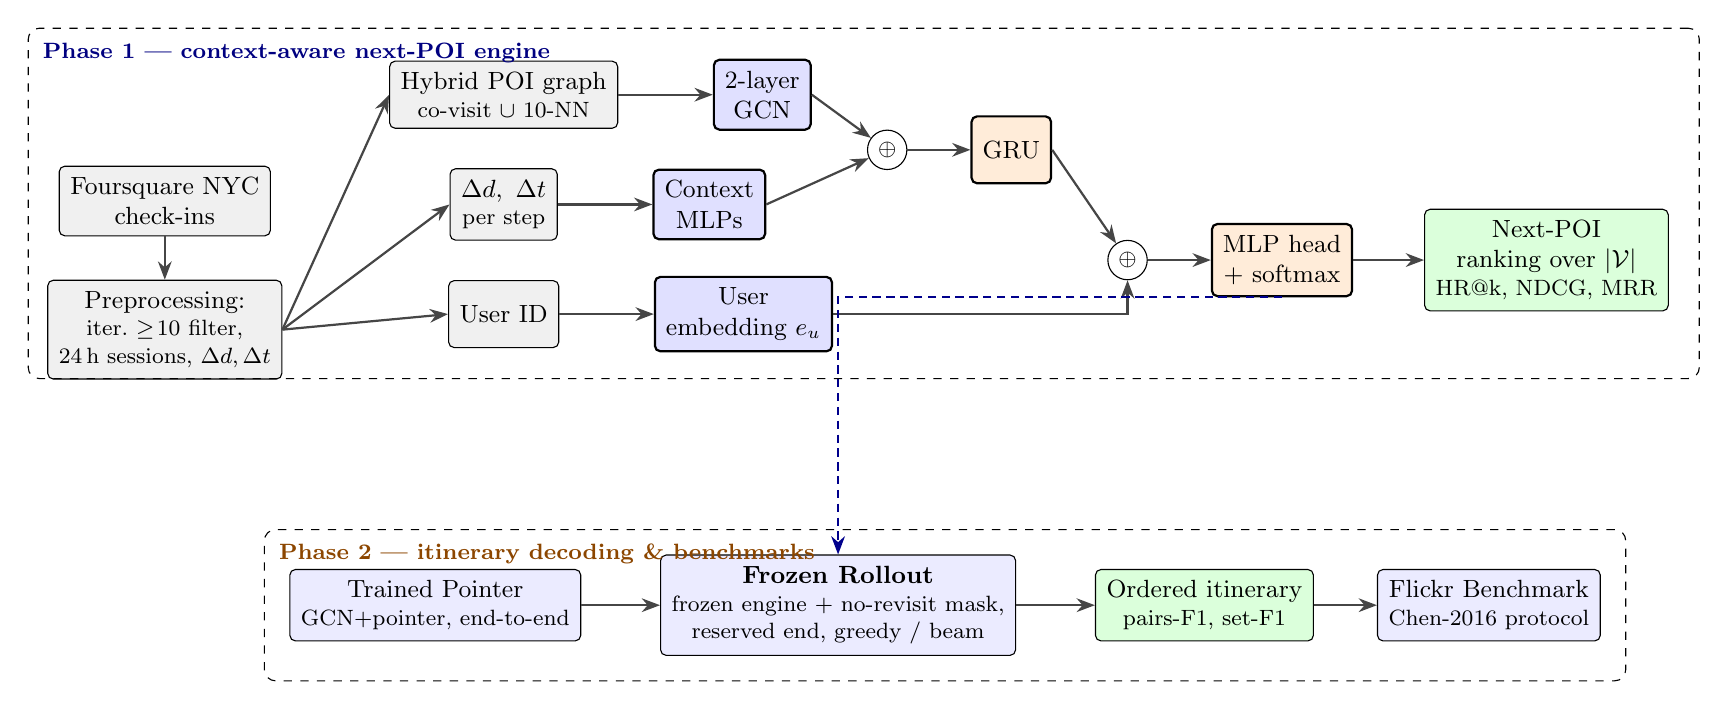
\begin{tikzpicture}[
    >=Stealth,
    font=\small,
    io/.style   ={draw, rounded corners=2pt, fill=gray!12, align=center, minimum height=0.85cm, inner sep=4pt},
    enc/.style  ={draw, rounded corners=2pt, fill=blue!12, thick, align=center, minimum height=0.85cm, inner sep=4pt},
    core/.style ={draw, rounded corners=2pt, fill=orange!15, thick, align=center, minimum height=0.85cm, inner sep=4pt},
    term/.style ={draw, rounded corners=2pt, fill=green!14, align=center, minimum height=0.85cm, inner sep=4pt},
    dec/.style  ={draw, rounded corners=2pt, fill=blue!8, align=center, minimum height=0.85cm, inner sep=4pt},
    merge/.style ={draw, circle, fill=white, inner sep=1pt, minimum size=0.5cm, font=\footnotesize},
    arr/.style  ={->, thick, gray!55!black},
]

% ---- Inputs / preprocessing ----
\node[io] (data) at (0,0) {Foursquare NYC\\check-ins};
\node[io, below=0.55cm of data] (prep) {Preprocessing:\\[-1pt]\footnotesize iter.\ $\ge\!10$ filter,\\[-1pt]\footnotesize 24\,h sessions, $\Delta d,\Delta t$};

% ---- Three encoder branches ----
\node[io,  right=1.5cm of data.east, yshift=1.35cm] (graph) {Hybrid POI graph\\[-1pt]\footnotesize co-visit $\cup$ 10-NN};
\node[io,  below=0.5cm of graph] (ctxin) {$\Delta d,\ \Delta t$\\[-1pt]\footnotesize per step};
\node[io,  below=0.5cm of ctxin] (userid) {User ID};

\node[enc, right=1.2cm of graph]  (gcn)  {2-layer\\GCN};
\node[enc, right=1.2cm of ctxin]  (cmlp) {Context\\MLPs};
\node[enc, right=1.2cm of userid] (uemb) {User\\embedding $e_u$};

% ---- Merge POI features + context, feed GRU ----
\node[merge, right=0.7cm of gcn, yshift=-0.7cm] (cat1) {$\oplus$};
\node[core, right=0.8cm of cat1] (gru) {GRU};
\node[merge, right=0.7cm of gru, yshift=-1.4cm] (cat2) {$\oplus$};
\node[core, right=0.8cm of cat2] (head) {MLP head\\+ softmax};
\node[term, right=0.9cm of head] (nextpoi) {Next-POI\\ranking over $|\mathcal{V}|$\\[-1pt]\footnotesize HR@k, NDCG, MRR};

% ---- Arrows: Phase 1 ----
\draw[arr] (data) -- (prep);
\draw[arr] (prep.east) -- (graph.west);
\draw[arr] (prep.east) -- (ctxin.west);
\draw[arr] (prep.east) -- (userid.west);
\draw[arr] (graph) -- (gcn);
\draw[arr] (ctxin) -- (cmlp);
\draw[arr] (userid) -- (uemb);
\draw[arr] (gcn.east)  -- (cat1);
\draw[arr] (cmlp.east) -- (cat1);
\draw[arr] (cat1) -- (gru);
\draw[arr] (gru.east) -- (cat2);
\draw[arr] (uemb.east) -| (cat2);
\draw[arr] (cat2) -- (head);
\draw[arr] (head) -- (nextpoi);

% ---- Phase 2: itinerary decoding ----
\node[dec, below=4.7cm of gru, xshift=-2.2cm] (rollout)
  {\textbf{Frozen Rollout}\\[-1pt]\footnotesize frozen engine + no-revisit mask,\\[-1pt]\footnotesize reserved end, greedy / beam};
\node[dec, left=1.0cm of rollout] (pointer)
  {Trained Pointer\\[-1pt]\footnotesize GCN+pointer, end-to-end};
\node[term, right=1.0cm of rollout] (itin)
  {Ordered itinerary\\[-1pt]\footnotesize pairs-F1, set-F1};
\node[dec, right=0.8cm of itin] (flickr)
  {Flickr Benchmark\\[-1pt]\footnotesize Chen-2016 protocol};

\draw[arr, blue!55!black, densely dashed] (head.south) -| (rollout.north);
\draw[arr] (pointer) -- (rollout);
\draw[arr] (rollout) -- (itin);
\draw[arr] (itin) -- (flickr);

% ---- Phase containers (dashed fit boxes, no fill so they sit over the main layer) ----
\node[draw, dashed, rounded corners, inner sep=11pt, label={[anchor=north west,font=\footnotesize\bfseries,text=blue!50!black,xshift=2pt,yshift=-2pt]north west:Phase 1 --- context-aware next-POI engine},
      fit=(data)(graph)(gcn)(gru)(head)(nextpoi)(userid)] (p1box) {};
\node[draw, dashed, rounded corners, inner sep=9pt, label={[anchor=north west,font=\footnotesize\bfseries,text=orange!55!black,xshift=2pt,yshift=-2pt]north west:Phase 2 --- itinerary decoding \& benchmarks},
      fit=(pointer)(rollout)(itin)(flickr)] (p2box) {};

\end{tikzpicture}%
}
\caption{Architecture of the proposed system. \textbf{Phase~1} (the next-POI engine): a
two-layer GCN over a hybrid POI graph (training-set co-visitation edges $\cup$ geographic
10-nearest-neighbour edges) produces POI features; per-step spatial/temporal gaps
$(\Delta d,\Delta t)$ are lifted by small MLPs; a learnable user embedding $e_u$ encodes
identity. The concatenated POI-feature/context sequence is read by a GRU, whose final state
is concatenated with $e_u$ and scored by an MLP head over the full POI vocabulary
($\mathrm{HR@}k$, $\mathrm{NDCG@}k$, $\mathrm{MRR}$). \textbf{Phase~2} (itinerary
recommendation): the \emph{frozen} engine is decoded into ordered routes by \emph{Frozen
Rollout} (no-revisit mask, reserved end POI, greedy or beam), compared against an end-to-end
\emph{Trained Pointer}; both are scored with set-F1 / pairs-F1 and validated on the Flickr
datasets under the Chen-2016 protocol.}
\label{fig:pipeline-overview}
\end{figure}


\textbf{Phase~1 --- the next-POI engine.} Raw Foursquare check-ins are filtered and grouped
into per-user sessions, and each consecutive visit pair is annotated with its spatial gap
$\Delta d$ (haversine distance) and temporal gap $\Delta t$ (elapsed time). A two-layer Graph
Convolutional Network (GCN) over a hybrid POI graph produces a feature vector for every POI;
the GCN features and the per-step context $(\Delta d,\Delta t)$ form the input to a GRU, whose
final state is combined with a learnable user embedding and scored by a multilayer-perceptron
(MLP) head over the full POI vocabulary. The engine is trained for single-step next-POI
prediction and evaluated with ranking metrics ($\mathrm{HR@}k$, $\mathrm{NDCG@}k$,
$\mathrm{MRR}$).

\textbf{Phase~2 --- itinerary decoding.} Given a query (a user, a start POI, an optional end
POI, and a desired length), \emph{Frozen Rollout} rolls the frozen engine forward, masking
already-visited POIs and reserving the final step for the end POI, to produce an ordered route.
As an integrated alternative, a \emph{Trained Pointer} replaces the MLP head with an
attention-style pointer and is trained end-to-end on whole trajectories. Itineraries are scored
with set-F1 and order-aware pairs-F1, and---because the Foursquare numbers are not on the same
scale as the published trip-recommendation literature---are re-validated on the Flickr
photo-trajectory datasets under the exact protocol of Chen et al.~\cite{chen2016learning}.

% ============================================================
\section{Data Preparation}
\label{sec:sol-data}
% ============================================================

\subsection{Filtering and sessionization}
\label{sec:sol-data-filter}

We use the standard Foursquare NYC check-in dataset of Yang et al.~\cite{yang2015foursquare}
($\sim$227K check-ins, $\sim$1.08K users, $\sim$38K venues). As is standard in next-POI
research, the raw data is reduced to a denser, more learnable core by an \emph{iterative
$k$-core filter}: users with fewer than ten check-ins and POIs with fewer than ten check-ins
are removed, and the procedure is repeated until the set is stable (in practice a few
iterations). This retains roughly $5{,}100$ POIs and $\sim$1.0K users. We deliberately keep
this filter simple and reproducible; a tourism-specific semantic curation of the catalogue is
discussed as future work (Chapter~\ref{ch:conclusion}).

User and POI identifiers are re-indexed to contiguous integers. Check-ins are then grouped
into \textbf{sessions}: a gap of more than 24~hours between successive check-ins of the same
user starts a new session, and sessions of length one (which admit no prediction) are dropped.

\subsection{Spatial and temporal gap features}
\label{sec:sol-data-context}

For every consecutive pair of check-ins within a session we compute two context scalars: the
\textbf{spatial gap} $\Delta d_t$ (haversine distance in km from the previous POI, clipped to
$[0,100]$) and the \textbf{temporal gap} $\Delta t_t$ (elapsed time in hours, clipped to
$[0,24]$). At the first step of a session $\Delta d_1=\Delta t_1=0$. These two gaps are the
\emph{only} contextual signals the engine consumes; they capture how far and how long a user
moved between visits, which is the spatio-temporal regularity exploited by ST-RNN-style models
\cite{liu2016strnn}. Time-of-day and weather are not modelled.

\subsection{Hybrid POI graph}
\label{sec:sol-data-graph}

To let the model reason about POIs beyond their individual identity, we build a single
undirected \textbf{hybrid graph} $G=(\mathcal{V},\mathcal{E}_{\mathrm{cov}}\cup
\mathcal{E}_{\mathrm{geo}})$ on the curated catalogue:
\begin{itemize}[leftmargin=*]
  \item \textbf{Co-visitation edges} $\mathcal{E}_{\mathrm{cov}}$: an edge $(p_i,p_j)$ is added
        when at least three consecutive $p_i\!\rightarrow\!p_j$ transitions occur within the
        \emph{training} sessions, encoding behavioural proximity;
  \item \textbf{Geographic edges} $\mathcal{E}_{\mathrm{geo}}$: each POI is connected to its
        ten nearest neighbours by haversine distance (computed with a ball tree), encoding
        spatial proximity.
\end{itemize}
The two edge sets are unioned and symmetrized. Co-visitation edges are derived from training
data only, so no test information leaks into the graph.

\subsection{Splitting}
\label{sec:sol-data-split}

Sessions are split \textbf{chronologically per user} into 70\%/10\%/20\% train/validation/test,
so that no future session of a user is used to predict its past. This split is shared by the
next-POI evaluation and (its test portion) by the NYC itinerary evaluation.

% ============================================================
\section{The Next-POI Engine}
\label{sec:sol-model}
% ============================================================

The engine maps a session prefix $S_u=(p_1,\dots,p_T)$ and its user $u$ to a probability
distribution over the next POI. It has four learnable parts: a graph encoder, a context
encoder, a user embedding, and a recurrent scorer. Default dimensions are
$d_p\!=\!128$ (POI), $d_u\!=\!64$ (user), $d_c\!=\!32$ (context), and $d_h\!=\!128$ (GRU hidden).

\subsection{Graph encoder}
\label{sec:sol-model-gcn}

A two-layer GCN over the hybrid graph transforms a learnable POI embedding table
$E^{(0)}\in\mathbb{R}^{|\mathcal{V}|\times d_p}$ into graph-aware POI features:
\begin{equation}
  E^{(l+1)} = \sigma\!\left(\tilde{D}^{-1/2}\,\tilde{A}\,\tilde{D}^{-1/2}\,E^{(l)}\,W^{(l)}\right),
  \qquad l = 0,1,
  \label{eq:gcn}
\end{equation}
where $\tilde{A}=A+I$ is the adjacency with self-loops, $\tilde{D}$ its degree matrix,
$\sigma$ a ReLU non-linearity (with dropout between layers), and $W^{(l)}$ the layer weights.
The POI feature used downstream is $h_p^{\mathrm{GCN}}=E^{(2)}_p\in\mathbb{R}^{d_p}$. Because the
graph is fixed, the full forward pass of Eq.~\eqref{eq:gcn} is computed \emph{once} per batch
(and once per decode) and indexed for each POI in a sequence.

\subsection{Context encoder}
\label{sec:sol-model-context}

The two gap scalars are lifted to a $d_c$-dimensional context vector by two small MLPs and
concatenated:
\begin{equation}
  c_t = \big[\,\mathrm{MLP}_d(\Delta d_t)\;\Vert\;\mathrm{MLP}_t(\Delta t_t)\,\big]
        \in\mathbb{R}^{d_c}.
  \label{eq:context}
\end{equation}

\subsection{User embedding}
\label{sec:sol-model-user}

User identity is encoded by a learnable embedding lookup $e_u\in\mathbb{R}^{d_u}$. This is a
collaborative, identity-based representation learned from the user's own visit history during
training; it is not derived from a persona description. The contribution of this embedding is
isolated by a dedicated ablation in Section~\ref{sec:sol-results-pers}.

\subsection{Recurrent scorer and output}
\label{sec:sol-model-gru}

At each step the GCN feature and the context are concatenated,
$x_t=[\,h_{p_t}^{\mathrm{GCN}}\;\Vert\;c_t\,]\in\mathbb{R}^{d_p+d_c}$, and the sequence
$X=(x_1,\dots,x_T)$ is read by a GRU. Its final hidden state $h_T\in\mathbb{R}^{d_h}$ is
concatenated with the user embedding and scored by an MLP head over the whole vocabulary:
\begin{align}
  h_T &= \mathrm{GRU}(x_1,\dots,x_T), \qquad z = [\,h_T\;\Vert\;e_u\,], \label{eq:gru}\\
  \hat{y} &= W_2\,\mathrm{ReLU}(W_1 z + b_1) + b_2 \in \mathbb{R}^{|\mathcal{V}|}, \label{eq:head}\\
  P(p_{T+1}&=p_j\mid S_u,u) = \frac{\exp(\hat{y}_j)}{\sum_k \exp(\hat{y}_k)}.
\end{align}
The model is trained by minimizing the next-POI cross-entropy over all session prefixes:
\begin{equation}
  \mathcal{L} = -\frac{1}{N}\sum_{i=1}^{N}\log P\!\left(y^{(i)}\mid S_u^{(i)},u^{(i)}\right),
  \label{eq:loss}
\end{equation}
with the Adam optimizer, gradient clipping, dropout regularization, and early stopping on
validation $\mathrm{HR@}10$. A session of length $L$ contributes $L-1$ prefix/target training
pairs, giving dense supervision (on the order of $10^5$ examples on NYC).

% ============================================================
\section{From Next-POI Scores to Itineraries}
\label{sec:sol-decoding}
% ============================================================

\subsection{Problem and query}
\label{sec:sol-decoding-query}

Itinerary recommendation takes a query $q=(u,s,e,K)$---a user $u$, a start POI $s$, an
optional end POI $e$, and a length budget $K$---and returns an ordered, loop-free route
$\hat{Y}=(s,p_2,\dots,e)$ of length $K$. Following the Chen-2016 convention
\cite{chen2016learning}, the start, the end, and the length are \emph{given}, and quality is
how well $\hat{Y}$ recovers the user's actual visited sequence $Y$. We use the length budget
(read directly as the ground-truth session length) as the headline mode, because it needs no
invented travel-speed or dwell-time constants and is therefore fully reproducible.

\subsection{Frozen Rollout (the headline method)}
\label{sec:sol-decoding-rollout}

The key observation is that the Phase-1 engine already scores a distribution over the next POI
for any partial route. An itinerary is what we obtain by \emph{rolling that scorer out} under
two constraints it never saw at training time:
\begin{enumerate}[label=(\roman*),leftmargin=*]
  \item \textbf{No-revisit mask}: the logit of every already-visited POI is set to $-\infty$,
        enforcing loop-free routes \cite{menon2017revisits};
  \item \textbf{Reserved end}: at the final step the route is forced to the queried end POI
        $e$ (the discrete analogue of the orienteering start/end constraint).
\end{enumerate}
\emph{Nothing in the trained model changes}---the same checkpoint serves both tasks; the entire
itinerary capability is an inference-time decoder. Two decoders are used: \textbf{greedy}
(take the \texttt{argmax} of the masked logits at each step) as the deterministic floor, and
\textbf{beam($b$)} (keep the $b$ partial routes with the highest summed transition
log-probability). At decode time $\Delta d$ is the real haversine distance between consecutive
route POIs and $\Delta t$ is a single documented constant; in length-budget mode this constant
affects only the context features, not the stop rule. Crucially, this headline decoder uses
\emph{no} travel-cost penalty and \emph{no} diversity bonus---augmenting the beam objective
with such penalties is left to future work (Chapter~\ref{ch:conclusion}).

\subsection{Trained Pointer (the integrated alternative)}
\label{sec:sol-decoding-pointer}

To test whether a model trained \emph{directly} for itineraries beats the decoded engine, we
also implement a pointer-network decoder \cite{vinyals2015pointer}. It reuses the GCN encoder
and user embedding but replaces the fixed MLP head with an \textbf{inner-product pointer}:
the decoder state $h_t$ is projected and scored against every POI feature,
$\mathrm{logit}_v=\langle W_o[h_t\Vert e_u],\,h_v^{\mathrm{GCN}}\rangle$, tying the output
directly to the graph signal. It is trained with teacher-forced sequence cross-entropy over
\emph{whole} length-$\ge\!3$ trajectories (one example per session), with the no-revisit mask
applied only at decode time and early stopping on validation pairs-F1. A context-aware variant
additionally feeds the $(\Delta d,\Delta t)$ context at each decoder step. Because each session
yields a single whole-trajectory example, the pointer sees far fewer updates than the
prefix-rich next-POI engine---a supervision-density gap that the results make visible.

% ============================================================
\section{Experimental Setup}
\label{sec:sol-experiments}
% ============================================================

\subsection{Two tasks, two benchmarks}
\label{sec:sol-exp-tasks}

This thesis evaluates two \emph{formally distinct} sub-tasks, each on its own field-standard
benchmark, following the surveys of Lim et al.~\cite{lim2018survey} and
Halder et al.~\cite{halder2024survey}:
\begin{itemize}[leftmargin=*]
  \item \textbf{Next-POI prediction} on Foursquare NYC, with full-vocabulary
        $\mathrm{HR@}k$/$\mathrm{NDCG@}k$/$\mathrm{MRR}$ (the protocol of GETNext
        \cite{yang2022getnext} and LLM4POI \cite{li2024llm4poi});
  \item \textbf{Itinerary recommendation} with set-F1 and pairs-F1, reported both internally on
        Foursquare NYC and---for literature comparison---on the Flickr photo-trajectory cities
        under the Chen-2016 protocol \cite{chen2016learning}.
\end{itemize}
The two tasks' metrics are \textbf{not on a common scale and are never cross-compared}: a
next-POI $\mathrm{HR@}1$ and an itinerary pairs-F1 measure different things, and absolute scores
across datasets with different POI-vocabulary sizes are not comparable
\cite{krichene2020sampled}. This is why the NYC itinerary numbers (Section~\ref{sec:sol-results-nyc})
and the Flickr numbers (Section~\ref{sec:sol-results-flickr}) live in separate tables.

\subsection{Metrics}
\label{sec:sol-exp-metrics}

\textbf{Next-POI:} $\mathrm{HR@}k$ (the true next POI is ranked in the top $k$ of the full
vocabulary), $\mathrm{NDCG@}k$, and $\mathrm{MRR}$, all without sampled negatives.

\textbf{Itinerary:} for a route, let its ordered-pair set be
$P(T)=\{(T_i,T_j):i<j\}$. Then
$\text{pairs-F1}$ is the F1 over $P(\hat{Y})$ vs $P(Y)$ (a pair counts only if both POIs appear
in both routes \emph{in the same order}), and $\text{set-F1}$ is the order-agnostic F1 over the
visited \emph{sets}. We report both, plus the exact-match rate. The pairs-F1 implementation is
pinned by unit tests against the Chen-2016 reference, and---per the faithfulness rule below---a
\texttt{Random} baseline reproduces Chen's published \texttt{Random} within noise. Following the
literature, itinerary metrics are reported on \textbf{length-$\ge\!3$, loop-free} trajectories,
where pairs-F1 has dynamic range (length-2 queries are trivial $s\!\to\!e$ recoveries).

\subsection{Baselines}
\label{sec:sol-exp-baselines}

For \emph{next-POI}, we position the engine against the published tier from the LLM4POI
benchmark table (LSTM, STGCN \cite{yu2018stgcn}, STAN \cite{luo2021stan}, GETNext
\cite{yang2022getnext}, STHGCN \cite{yan2023sthgcn}, LLM4POI \cite{li2024llm4poi}). For the
\emph{itinerary} task, the NYC study contrasts Frozen Rollout against the Trained Pointer, and
the Flickr Benchmark adds classical baselines (\texttt{Random}, \texttt{PoiPopularity},
\texttt{Markov}, \texttt{MarkovPath}) and the published methods PoiRank/Rank+Markov
\cite{chen2016learning}, DeepTrip \cite{gao2019deeptrip}, CTLTR \cite{zhou2021ctltr}, SelfTrip
\cite{gao2022selftrip}, and AR-Trip \cite{shu2024artrip}.

% ============================================================
\section{Results and Discussion}
\label{sec:sol-results}
% ============================================================

\subsection{Next-POI accuracy (Phase~1)}
\label{sec:sol-results-nextpoi}

Table~\ref{tab:nextpoi} reports the engine's full-vocabulary ranking accuracy on Foursquare
NYC. The model reaches $\mathrm{HR@}1=0.187$, i.e.\ the exact next venue is the top prediction
out of $\sim$5{,}100 candidates almost one time in five, with $\mathrm{MRR}=0.316$.

\begin{table}[ht]
\centering
\caption{Next-POI prediction accuracy of the proposed engine on Foursquare NYC
(full vocabulary, test set).}
\label{tab:nextpoi}
\begin{tabular}{lcccccc}
\toprule
Model & HR@1 & HR@5 & HR@10 & NDCG@5 & NDCG@10 & MRR \\
\midrule
Ours (GCN+GRU+user) & 0.187 & 0.476 & 0.588 & 0.339 & 0.375 & 0.316 \\
\bottomrule
\end{tabular}
\end{table}

To position this honestly, Table~\ref{tab:nextpoi-tier} places our $\mathrm{HR@}1$ within the
published tier (numbers as collated in the LLM4POI benchmark). The engine sits in the
\emph{LSTM/STGCN band}: clearly learning (well above an LSTM and on par with a spatio-temporal
GCN) but below the attention/transformer SOTA (STAN, GETNext, STHGCN) and far below the
LLM-based LLM4POI. This is the expected, defensible position for a compact GCN+GRU model and is
stated as such rather than overclaimed.

\begin{table}[ht]
\centering
\caption{$\mathrm{HR@}1$ (equivalently $\mathrm{Acc@}1$) tier on Foursquare NYC, as collated in
the LLM4POI benchmark. Our engine is in bold.}
\label{tab:nextpoi-tier}
\begin{tabular}{lc}
\toprule
Model & HR@1 \\
\midrule
LSTM & 0.130 \\
STGCN~\cite{yu2018stgcn} & 0.180 \\
\textbf{Ours (GCN + GRU + user)} & \textbf{0.187} \\
STAN~\cite{luo2021stan} & 0.220 \\
GETNext~\cite{yang2022getnext} & 0.240 \\
STHGCN~\cite{yan2023sthgcn} & 0.270 \\
LLM4POI~\cite{li2024llm4poi} & 0.340 \\
\bottomrule
\end{tabular}
\end{table}

\subsection{Itinerary on NYC: Frozen Rollout vs.\ Trained Pointer}
\label{sec:sol-results-nyc}

Table~\ref{tab:nyc-itin} reports the headline integration experiment on the NYC test sessions
($n=2{,}880$ length-$\ge\!3$ trajectories). The result is deliberately counter-intuitive:
\textbf{decoding the frozen next-POI engine (decoupled) beats the purpose-trained pointer
(integrated)} by about $0.03$ pairs-F1 ($-10.5\%$ for the pointer). Beam search barely improves
on greedy ($+0.0015$ pairs-F1), which shows the limitation is the engine's myopia, not the
decoder: smarter search cannot recover information the scorer never had.

\begin{table}[ht]
\centering
\caption{Itinerary recommendation on Foursquare NYC (length-$\ge\!3$ test, $n=2{,}880$). Higher
is better; itinerary metrics are \emph{not} comparable to the next-POI metrics of
Table~\ref{tab:nextpoi}.}
\label{tab:nyc-itin}
\begin{tabular}{llccc}
\toprule
Method & Type & pairs-F1 & set-F1 & exact \\
\midrule
\textbf{Frozen Rollout} (greedy) & decoupled & \textbf{0.289} & 0.609 & 0.054 \\
Frozen Rollout (beam~3) & decoupled & 0.290 & 0.610 & 0.057 \\
Trained Pointer v1 (no context) & integrated & 0.259 & 0.578 & 0.043 \\
Trained Pointer v2 (\,+\,context) & integrated & 0.261 & --- & --- \\
\bottomrule
\end{tabular}
\end{table}

The pointer trained cleanly (validation pairs-F1 rising to a genuine peak before early
stopping), so this is a real negative result, not a bug. Three factors explain why the simpler
route wins: (i)~\textbf{supervision density}---the engine learns from $\sim$$10^5$ prefix/target
pairs (every prefix of every session), whereas the pointer sees only one whole-trajectory
example per session; (ii)~\textbf{leaner inputs}---the v1 pointer conditions only on the
previous POI's graph feature, which is why adding the $(\Delta d,\Delta t)$ context in v2
recovers a small amount; and (iii)~\textbf{converged vs.\ from-scratch}---Frozen Rollout reuses
a fully-trained engine while the pointer trains its encoder from random initialization. The
takeaway for the thesis is that \emph{naively training a dedicated itinerary model does not
automatically beat cleverly decoding a strong next-POI model}---a nuance to the integration
narrative of Halder et al.~\cite{halder2025drlir}.

A second, important caveat is that these NYC pairs-F1 values ($\approx0.26$--$0.29$) are
\textbf{not comparable} to the published trip-recommendation numbers ($\approx0.6$--$0.85$):
the published works evaluate on Flickr cities of $\sim$25--90 POIs, whereas NYC has $\sim$5{,}100
POIs, so the chance level differs by two orders of magnitude. The gap is a dataset/vocabulary
artifact, not a quality gap---which is precisely why the next subsection re-runs the task on the
literature's own benchmark.

\subsection{The Flickr Benchmark (literature-comparable)}
\label{sec:sol-results-flickr}

To place the itinerary task on the same scale as the published literature, we re-run it on the
five Flickr photo-trajectory cities under the \emph{exact} Chen-2016 protocol
\cite{chen2016learning}: leave-one-trajectory-out cross-validation, the query gives the first
and last POI plus the desired length, and evaluation is on length-$\ge\!3$ loop-free
trajectories. Table~\ref{tab:flickr-data} lists the datasets.

\begin{table}[ht]
\centering
\caption{Flickr photo-trajectory datasets (canonical Chen-2016 files). Evaluation is on the
length-$\ge\!3$ subset.}
\label{tab:flickr-data}
\begin{tabular}{lcccc}
\toprule
City & \#POIs & \#users & \#trajectories & \#traj.\ (len $\ge 3$) \\
\midrule
Toronto   & 29 & 1{,}395 & 6{,}057 & 335 \\
Osaka     & 27 &   450 & 1{,}115 &  47 \\
Glasgow   & 27 &   601 & 2{,}227 & 112 \\
Edinburgh & 28 & 1{,}454 & 5{,}028 & 634 \\
Melbourne & 88 & 1{,}000 & 5{,}106 & 442 \\
\bottomrule
\end{tabular}
\end{table}

\paragraph{Protocol faithfulness.} A \texttt{Random} baseline has no modelling choices, so it
must reproduce Chen's \texttt{Random} if and only if the data, protocol, and metric are
identical. Table~\ref{tab:flickr-faith} shows they match within noise (and our
\texttt{PoiPopularity} matches Chen's near-exactly on the data-rich cities), which validates
that our harness is protocol-faithful---a prerequisite for any comparison to the literature.

\begin{table}[ht]
\centering
\caption{Faithfulness check (pairs-F1): our reproductions vs.\ Chen 2016.}
\label{tab:flickr-faith}
\begin{tabular}{llccccc}
\toprule
Method & Source & Toronto & Osaka & Glasgow & Edinburgh & Melbourne \\
\midrule
\multirow{2}{*}{Random} & ours & 0.298 & 0.301 & 0.301 & 0.270 & 0.227 \\
                        & Chen 2016 & 0.310 & 0.304 & 0.320 & 0.261 & 0.248 \\
\addlinespace
\multirow{2}{*}{PoiPopularity} & ours & 0.443 & 0.413 & 0.510 & 0.439 & 0.320 \\
                               & Chen 2016 & 0.384 & 0.365 & 0.507 & 0.436 & 0.316 \\
\bottomrule
\end{tabular}
\end{table}

\paragraph{Our results.} Table~\ref{tab:flickr-ours} reports our classical baselines and the
learned pointer. The headline is that \textbf{our pairs-F1 now spans $0.23$--$0.59$, on the
published $0.26$--$0.85$ scale}, versus $0.26$--$0.29$ on NYC---confirming that the low NYC
numbers were a property of the data and protocol, not the method. Among our methods the
first-order \texttt{Markov} transition baseline is strongest, and the light from-scratch pointer
(0.31--0.49) reaches the scale and beats \texttt{Random} comfortably but trails \texttt{Markov}
on every city---the same supervision-density lesson seen on NYC.

\begin{table}[ht]
\centering
\caption{Our itinerary results on the Flickr cities (pairs-F1, leave-one-out, length $\ge 3$).}
\label{tab:flickr-ours}
\begin{tabular}{lccccc}
\toprule
Method & Toronto & Osaka & Glasgow & Edinburgh & Melbourne \\
\midrule
Random        & 0.298 & 0.301 & 0.301 & 0.270 & 0.227 \\
PoiPopularity & 0.443 & 0.413 & 0.510 & 0.439 & 0.320 \\
Markov (greedy) & \textbf{0.504} & \textbf{0.421} & \textbf{0.587} & 0.449 & 0.333 \\
MarkovPath (beam) & 0.528 & 0.398 & 0.543 & \textbf{0.452} & \textbf{0.346} \\
Pointer (learned, beam~3) & 0.431 & 0.399 & 0.489 & 0.414 & 0.312 \\
\bottomrule
\end{tabular}
\end{table}

\paragraph{Comparison to the literature.} Table~\ref{tab:flickr-pub} lists the directly
comparable published pairs-F1 (same protocol, same $0$--$1$ scale). Our classical line lands
between the published classical methods (PoiRank, Rank+Markov) on several cities, while the
neural SOTA (DeepTrip, CTLTR, SelfTrip, AR-Trip) reaches $0.66$--$0.85$ using machinery our
light model omits: self-supervised and contrastive pre-training, trajectory augmentation, and
adversarial training. There is no single SOTA across all cities: AR-Trip leads on
Toronto, Glasgow and Edinburgh, while SelfTrip is best on Osaka.

\begin{table}[ht]
\centering
\caption{Published, directly-comparable itinerary pairs-F1 on the Flickr cities (same Chen-2016
protocol). ``cl.''~=~classical, ``ne.''~=~neural.}
\label{tab:flickr-pub}
\begin{tabular}{llcccc}
\toprule
Method & Fam. & Toronto & Osaka & Glasgow & Edinburgh \\
\midrule
PoiRank~\cite{chen2016learning}      & cl. & 0.518 & 0.511 & 0.548 & 0.432 \\
Rank+Markov~\cite{chen2016learning}  & cl. & 0.512 & 0.486 & 0.545 & 0.444 \\
DeepTrip~\cite{gao2019deeptrip}      & ne. & 0.748 & 0.755 & 0.782 & 0.660 \\
CTLTR~\cite{zhou2021ctltr}           & ne. & 0.748 & 0.719 & 0.763 & 0.681 \\
SelfTrip~\cite{gao2022selftrip}      & ne. & 0.835 & \textbf{0.851} & 0.818 & 0.779 \\
AR-Trip~\cite{shu2024artrip}         & ne. & \textbf{0.839} & 0.828 & \textbf{0.820} & \textbf{0.808} \\
\bottomrule
\end{tabular}
\end{table}

\subsection{Personalization ablation}
\label{sec:sol-results-pers}

Because a per-user embedding is the system's only personalization mechanism, we isolate its
effect with a controlled ablation on the Flickr pointer (user embedding on vs.\ off; dimension
64, 30 epochs, leave-one-out). Table~\ref{tab:pers} shows the effect is \textbf{mixed}: it helps
clearly on Glasgow ($+0.038$ pairs-F1) but is roughly neutral-to-slightly-negative on Osaka and
Toronto. The honest reading is that, under leave-one-trajectory-out on these small datasets, most
users contribute too few trajectories for an identity embedding to be reliably estimated
(a cold-start effect); personalization helps only where user signal is both present and
consistent. The two larger cities (Edinburgh, Melbourne) are deferred to a GPU run.

\begin{table}[ht]
\centering
\caption{Personalization ablation: pointer pairs-F1 \emph{without} vs.\ \emph{with} the user
embedding (Flickr, length $\ge 3$, dim 64, 30 epochs).}
\label{tab:pers}
\begin{tabular}{lccc}
\toprule
City & no user emb. & + user emb. & $\Delta$ \\
\midrule
Glasgow & 0.451 & 0.489 & $+0.038$ \\
Osaka   & 0.442 & 0.435 & $-0.007$ \\
Toronto & 0.440 & 0.423 & $-0.017$ \\
\bottomrule
\end{tabular}
\end{table}

\subsection{Discussion}
\label{sec:sol-results-discussion}

The experiments support three honest conclusions, one per research question.
\textbf{(RQ1)} A learnable user embedding is the realized personalization mechanism; its benefit
is real but conditional (Glasgow $+0.038$), not universal---tourism's cold-start sparsity limits
identity-based personalization, motivating the persona/content-based direction as future work.
\textbf{(RQ2)} The spatial/temporal gap features $(\Delta d,\Delta t)$ and the hybrid POI graph
give the engine an honest LSTM/STGCN-tier accuracy ($\mathrm{HR@}1=0.187$); richer context such
as weather and time-of-day is a clear, but unrealized, extension.
\textbf{(RQ3)} A frozen next-POI engine can be decoded into coherent itineraries, and doing so
(Frozen Rollout) \emph{beats} a purpose-trained pointer because of its much denser supervision;
beam search alone cannot close the residual order gap (set-F1 $\gg$ pairs-F1), which points to
richer, constraint- and schedule-aware decoders (e.g.\ DLIR-style \cite{halder2025drlir}) as the
way forward. The Flickr Benchmark confirms that all of these conclusions sit on the literature's
own scale and that our harness reproduces Chen 2016, while honestly placing our light models
below the self-supervised neural SOTA.

% ============================================================
\section{Chapter Summary}
\label{sec:sol-summary}
% ============================================================

This chapter described the system as actually built: a context-aware next-POI engine (a GCN over
a hybrid POI graph, $(\Delta d,\Delta t)$ gap context, a user embedding, and a GRU scorer),
decoded into itineraries by Frozen Rollout and compared against an end-to-end Trained Pointer.
On Foursquare NYC the engine reaches an honest $\mathrm{HR@}1=0.187$, and---counter-intuitively
---decoding the frozen engine beats the integrated pointer ($0.289$ vs.\ $0.259$ pairs-F1).
On the Flickr Benchmark our methods land on the published $0.26$--$0.85$ scale with a
protocol-faithful harness (Random reproduces Chen 2016), our \texttt{Markov} baseline is strong,
and personalization is mixed. The next chapter draws these honest findings together and outlines
the unrealized extensions---weather/time context, persona-based cold-start, semantic curation,
and constraint-aware decoding---as future work.

\chapter{Conclusion and Perspectives}
\label{ch:conclusion}

% ============================================================
\section{Summary of Contributions}
\label{sec:conc-summary}
% ============================================================

This thesis addressed the problem of producing personalized tourist itineraries from check-in
data, and did so through a deliberately \emph{decoupled} design: a strong next-POI engine,
decoded into ordered routes. Its contributions, each tied to a research question, are:

\begin{enumerate}
  \item \textbf{A context-aware next-POI engine (RQ1, RQ2).} The engine combines a graph
  convolutional network over a hybrid POI graph (training-set co-visitation $\cup$ geographic
  neighbours), per-step spatial/temporal gap features $(\Delta d,\Delta t)$, a learnable user
  embedding, and a GRU scorer over the full POI vocabulary. On Foursquare NYC it reaches an
  honest $\mathrm{HR@}1=0.187$, placing it in the LSTM/STGCN tier---clearly learning, while
  below the transformer and LLM state of the art. A controlled ablation shows that the user
  embedding personalizes \emph{conditionally}: it helps where user signal is present and
  consistent (Glasgow, $+0.038$ pairs-F1) but is roughly neutral under the sparse,
  cold-start regime of the other cities.

  \item \textbf{Itinerary generation by Frozen Rollout, and an integration study (RQ3).} We
  obtain itineraries by rolling the \emph{frozen} engine forward under a no-revisit mask and a
  reserved end POI, changing nothing in the trained model. Against a purpose-trained
  pointer-network decoder (\emph{Trained Pointer}), the decoupled \emph{Frozen Rollout}
  \emph{wins} on NYC ($0.289$ vs.\ $0.259$ pairs-F1). The honest lesson---that a strongly
  (densely) supervised next-POI model is hard to beat by naively training a dedicated itinerary
  model---nuances the integration narrative of recent deep itinerary work.

  \item \textbf{A literature-comparable Flickr benchmark (validation).} Because the NYC
  itinerary scores are not on the same scale as the published trip-recommendation literature
  (a POI-vocabulary artifact, not a quality gap), we re-ran the task on the five Flickr
  photo-trajectory cities under the exact Chen-2016 protocol. A \texttt{Random} baseline
  reproduces Chen 2016 within noise---demonstrating protocol faithfulness---and our methods land
  on the published $0.26$--$0.85$ scale, with a strong first-order \texttt{Markov} baseline and a
  light learned pointer that reaches the scale but trails the neural state of the art.
\end{enumerate}

Across both phases, a methodological contribution is the strict separation of the two
sub-tasks: next-POI prediction (Foursquare, $\mathrm{HR@}k$/$\mathrm{MRR}$) and itinerary
recommendation (Flickr, set-F1/pairs-F1) are reported on their own benchmarks and never
cross-compared.

% ============================================================
\section{Limitations}
\label{sec:conc-limitations}
% ============================================================

Several limitations should be acknowledged honestly:

\begin{itemize}
  \item \textbf{Accuracy below the neural/LLM SOTA.} The engine's $\mathrm{HR@}1=0.187$ is an
  LSTM/STGCN-tier result; attention/transformer models (GETNext, STHGCN) and LLM-based methods
  (LLM4POI) score higher. The contribution is an honest, reproducible baseline, not a new SOTA.

  \item \textbf{Decoding cannot fix engine myopia.} Beam search barely improves on greedy
  ($+0.0015$ pairs-F1 on NYC), and the persistent set-F1\,$\gg$\,pairs-F1 gap (right places,
  wrong order) shows that the residual error is in the scorer, not the search.

  \item \textbf{Light learned models trail strong simple ones.} On both NYC (Trained Pointer
  $<$ Frozen Rollout) and Flickr (pointer $<$ Markov), purpose-trained models lose to simpler
  baselines---a supervision-density and data-size effect on these small datasets.

  \item \textbf{Limited context and personalization.} The realized context is only the
  $(\Delta d,\Delta t)$ gaps, with no weather or absolute time-of-day; personalization is a
  user embedding whose benefit is conditional. The decode-time $\Delta t$ is an assumed
  constant rather than an observed value.

  \item \textbf{Single Foursquare city and offline evaluation.} The next-POI engine is trained
  on NYC only, and all evaluation is offline against historical sequences; no user study or
  deployment was conducted.
\end{itemize}

% ============================================================
\section{Future Work}
\label{sec:conc-future}
% ============================================================

The audit of what was \emph{designed but not evaluated} maps directly onto a concrete research
agenda:

\begin{itemize}
  \item \textbf{Richer context.} Add explicit time-of-day and weather embeddings (and, where
  available, real rather than assumed inter-visit times), testing whether environmental context
  measurably improves next-POI accuracy and itinerary suitability.

  \item \textbf{Persona-based cold-start personalization.} Replace (or augment) the identity
  embedding with a content/persona encoder that derives a preference vector from explicit
  interests and POI semantic metadata, targeting the cold-start regime where the user embedding
  is weakest.

  \item \textbf{Tourism-specific data curation.} Move from the simple iterative $k$-core filter
  to a semantic curation of tourist-relevant venues (category taxonomy plus embedding-based
  refinement), and measure its effect on transition quality and bias.

  \item \textbf{Constraint- and schedule-aware decoding.} Augment the rollout beam objective
  with travel-cost penalties, diversity bonuses, and time-window/opening-hour constraints, and
  compare against richer scheduling-aware itinerary models (e.g.\ DLIR-style architectures
  \cite{halder2025drlir}). A complementary orienteering-problem / iterated-local-search solver
  over the learned scores was scoped but not implemented, and remains a useful upper-reference.

  \item \textbf{Closing the neural gap.} Reach the SelfTrip/AR-Trip band on Flickr with the
  machinery those methods use---self-supervised/contrastive pre-training on the unlabelled
  trajectories, trajectory augmentation, and adversarial training---rather than a light
  from-scratch pointer.

  \item \textbf{Multi-city generalization and deployment.} Validate across cities (transfer or
  city-agnostic POI representations) and conduct user studies within a deployed planning
  application.
\end{itemize}

% ============================================================
\section{Closing Remarks}
\label{sec:conc-closing}
% ============================================================

Tourist itinerary recommendation sits at the intersection of personalization, sequential
prediction, and constrained generation. This thesis showed that a compact, honestly-evaluated
next-POI engine---a graph encoder, spatial/temporal gap context, a user embedding, and a
recurrent scorer---can be decoded into coherent itineraries simply and effectively, and that
this decoupled route is a stronger baseline than it first appears: it beats a purpose-trained
itinerary model on Foursquare NYC and, on the Flickr benchmark, lands on the literature's own
scale with a protocol-faithful harness. By reporting both tasks on their proper benchmarks and
resisting the temptation to overclaim, the work offers a defensible foundation and a clear,
honest path toward a fuller scheduling- and context-aware itinerary module.


% --------------------
% Back matter
% --------------------
\backmatter
\bibliography{refs}


\end{document}
